% \documentclass[letterpaper, 10 pt, conference, twoside]{support/IEEEconf}
\pdfoutput=1
\documentclass[letterpaper, 10pt, journal, twoside]{support/IEEEtran}

\let\proof\relax
\let\endproof\relax
\let\example\relax
\let\endexample\relax
\let\labelindent\relax
\let\algorithm\relax
% Define commands for /* ... */ style comments
\newcommand{\cstart}{\Comment{/\*}}
\newcommand{\cend}{\Comment{\*/}}
\newcommand{\ccomment}[1]{\Comment{#1}}
\usepackage{makecell}
\usepackage{times}
\usepackage[pdftex]{graphicx}
\usepackage{graphicx}
\usepackage{subfigure}
\usepackage{amsmath,amssymb,amsopn,amstext,amsfonts}
\usepackage{cancel}
\usepackage[space]{cite}
\usepackage{siunitx}
\usepackage{soul}
\usepackage{cuted}
% \usepackage{caption}        % 使用之后图题是冒号，不是句号
\usepackage{lipsum,multicol}
\usepackage{stfloats}
% \usepackage{ulem}
\everymath{\displaystyle}
\usepackage{booktabs}
\usepackage{threeparttable}
\usepackage{amsthm}
\usepackage{xfrac}
\usepackage{balance}
\usepackage{color}
\usepackage{mathtools}
\DeclareMathOperator*{\med}{med}
\usepackage{tabularx}
\usepackage{bm}
\usepackage{diagbox}
\usepackage{float}
\usepackage{epstopdf}
\usepackage{url}
\usepackage{multirow}
\usepackage{array,booktabs}
\usepackage{multicol}
\usepackage{tikz}
\usepackage{tablefootnote}
%\usepackage{hyperref}[linkcolor=black,citecolor=black,urlcolor=black,colorlinks=true]
\usepackage[linkcolor=blue,citecolor=blue,urlcolor=black,colorlinks=true]{hyperref}
\usepackage{enumitem}
% \usepackage[ruled,vlined,linesnumbered]{algorithm2e}
\usepackage{algorithmic}
\usepackage{algorithm}
\usepackage{pifont}
\newcommand{\cmark}{\ding{51}}%
\newcommand{\xmark}{\ding{55}}%
\DeclareMathAlphabet\mathbfcal{OMS}{cmsy}{b}{n}

\newtheorem{theorem}{Theorem}
\newtheorem{corollary}{Corollary}
\newtheorem{lemma}{Lemma}
\renewcommand{\qedsymbol}{$\blacksquare$}
\newcolumntype{M}[1]{>{\centering\arraybackslash}m{#1}}

\soulregister\cite7
\soulregister\citep7
\soulregister\citet7
\soulregister\ref7
\soulregister\it7
\soulregister\pageref7

\bibliographystyle{support/IEEEtran}

\newcommand{\ann}[1]{%
	\begin{tikzpicture}[remember picture, baseline=-0.75ex]%
		\node[coordinate] (inText) {};%
	\end{tikzpicture}%
	\marginpar{%
		\renewcommand{\baselinestretch}{1.0}%
		\begin{tikzpicture}[remember picture]%
			\definecolor{orange}{rgb}{1,0.5,0}%
			\draw node[fill=red!20,rounded corners,text width=\marginparwidth] (inNote){\footnotesize#1};%
		\end{tikzpicture}%
	}%
	\begin{tikzpicture}[remember picture, overlay]%
		\draw[draw = orange, thick]
		([yshift=-0.2cm] inText)
		-| ([xshift=-0.2cm] inNote.west)
		-| (inNote.west);%
	\end{tikzpicture}%
}%

\usepackage{arydshln}
\graphicspath{{figures/}}
\DeclareGraphicsExtensions{.pdf,.png,.jpg,.eps}
\DeclareMathOperator{\atantwo}{atan2}
\DeclareMathOperator{\atan}{atan}
\DeclareMathOperator{\sign}{sign}
\DeclareMathOperator{\arctantwo}{arctan2}
\IEEEoverridecommandlockouts
%\overrideIEEEmargins

\title{Multi-UAV Cooperative Exploration with Minimally Overlapping Coverage}
%

\author{Gang Xu$^{1, \dagger}$, Xinyang Liu$^{1, \dagger}$, Qinhan Chen$^{1}$, Tao Liu$^{2}$, Shengbo Li$^{1}$, and Yong Liu$^{1,*}$%
\thanks{$^{1}$Gang Xu, Xinyang Liu, Qinhan Chen, and Yong Liu are with the Institute of Cyber-Systems and Control, Zhejiang University, Hangzhou 310027, China (e-mail: wuuya@zju.edu.cn).}%
\thanks{$^{*}$Yong Liu is the corresponding author (e-mail: yongliu@iipc.zju.edu.cn).}
\thanks{$^{\dagger}$Gang Xu and Xinyang Liu contributed equally to this work.} %
}


\begin{document}
\maketitle
\begin{abstract}
Decentralized multi-UAV autonomous exploration has excellent potential in large-scale complex scenarios such as search and rescue and environment mapping due to its ability to rapidly cover unknown spaces, especially when equipped with sensors with a wide sensing range. However, as the sensing range increases, the amount of information to be processed and the communication load grow dramatically, significantly straining the limited onboard computational resources. To address this problem, this letter proposes a decentralized multi-UAV cooperative exploration strategy based on LiDAR sensors. It enables UAVs to rapidly compute feasible target viewpoints from vast frontier voxels and efficiently allocate them through collaborative strategies. Furthermore, the proposed method reduces unnecessary map information sharing, effectively alleviating the communication burden among multiple UAVs. Extensive large-scale exploration experiments show that the proposed method improves exploration efficiency by 35\% compared to current state-of-the-art methods, demonstrating the effectiveness and practicality of the approach.
\end{abstract}

\vspace{-0.28cm}
\begin{IEEEkeywords}
Multi-UAV cooperation, motion planning, autonomous exploration in large-scale environments.
\end{IEEEkeywords}

\section{Introduction}
\label{sec:intro}

% [What is the question? Why is it important and worth studying? Background and motivation]
\IEEEPARstart{A}{utonomous} exploration is a fundamental problem in robotic applications such as industrial inspection \cite{ yoder2016autonomous, bircher2018receding, gao2023uav}, 3D reconstruction \cite{hepp2018plan3d, yan2021sampling, zhang2024soar}, and search and rescue \cite{erdelj2017help, schedl2021autonomous, zhang2022fast}. Its primary task is to utilize one or many autonomous mobile robots to efficiently map an unknown environment within a specified area as quickly as possible. Compared to unmanned ground vehicles (UGVs), unmanned aerial vehicles (UAVs), particularly quadrotors, offer significant advantages in autonomous exploration due to their agility and flexibility. However, the limited battery life of UAVs, communication constraints during the exploration process, and high computational costs present substantial challenges. As a result, autonomous exploration of large-scale and complex environments remains an open problem.

% [How others have approached this problem? What are the limitations of their approach?]
Recently, many research efforts have focused on autonomous exploration, aiming to enhance the exploration efficiency of autonomous mobile robots in complex unknown environments. 
For example, Zhang et al. \cite{zhang2024falcon} proposed a method for decomposing unknown spaces based on a connectivity graph and utilized a hierarchical planner to generate a coverage path for the entire exploration space. It served as global guidance for exploration and improved the efficiency of UAV exploration. 
Furthermore, researchers have employed LiDAR for exploration in unknown environments \cite{tang2023bubble, lindqvist2024tree},  aiming to improve exploration efficiency by fully leveraging the advantages of LiDAR's broad sensing range. 
However, the exploration capability of a single UAV in large-scale environments is still limited. Meanwhile, due to the UAV's limited battery life, it is challenging to ensure that a single UAV can complete the exploration of a designated area within its flight endurance.
In contrast, multi-UAV cooperation holds great potential for rapid exploration in large-scale unknown environments, as demonstrated by substantial studies \cite{cao2023representation, zhou2023racer, bartolomei2023fast, dong2024fast}. However, most current multi-UAV collaborative exploration efforts rely on visual sensors for environmental exploration. Due to their limited sensing range, achieving efficient exploration in large-scale scenarios remains challenging.
Thanks to the large FoV, employing LiDAR instead of visual sensors is one critical approach to enabling rapid exploration in large-scale unknown environments. However, as the sensing range increases, the computational overhead associated with candidate viewpoints and frontier information in each exploration iteration grows significantly, making it difficult for UAVs to respond quickly to new exploration decisions. Moreover, since LiDAR data is typically much more significant than visual sensors, this further exacerbates the communication burden between multiple UAVs, severely impacting the efficiency of multi-UAV collaborative exploration. As a result, the potential of LiDAR's wide FoV to enhance exploration efficiency remains underexploited.

% [How we solved the problem? Motivations?]
To address these issues, we present {MAPPER}, a novel \textbf{M}ulti-U\textbf{A}V coo\textbf{P}eration ex\textbf{P}loration strategy in larg\textbf{E}-scale envi\textbf{R}onments, which further leverages the advantages of LiDAR's large FoV to enhance exploration efficiency. 
We first propose an efficient viewpoint generation method that enables UAVs to quickly extract valid viewpoints as access targets from many frontier voxels. It effectively alleviates the information processing burden caused by the increased sensing range. The key idea is to rapidly identify the known free regions surrounding each frontier before sampling and then perform viewpoint sampling within the known free region, quickly selecting appropriate viewpoints as target viewpoints for the corresponding frontiers. Meanwhile, inspired by the dual-mode exploration strategy proposed in \cite{bartolomei2023fast}, we further improved the UAV viewpoint allocation strategy under different exploration modes, avoiding situations where allocated target viewpoints are too close, and UAVs oscillate back and forth between target viewpoints. In addition, to mitigate the communication burden between UAVs, we share only the necessary map information for collision avoidance without sharing the entire 3D map.

% [Describe the results and summarize contribution bullets]
To validate the proposed exploration algorithm, we compared it with two state-of-the-art multi-UAV collaborative exploration algorithms and conducted extensive simulations in large-scale complex environments of $10{,}000\text{ m}^2$, $40{,}000\text{ m}^2$, and $90{,}000\text{ m}^2$, respectively. We also performed extensive hardware-in-the-loop experiments in the large-scale scenario of $10{,}000\text{ m}^2$. The experimental results demonstrate that the proposed MAPPER has significant advantages in both computational efficiency and fast exploration and can adapt to severely constrained communication conditions. The main contributions of this work are summarized as follows:
\begin{enumerate}
  \item An efficient viewpoint generation strategy for quickly processing frontier information enables rapid responses for UAVs and fully exploits the potential of LiDAR's wide field of view (FoV).
  \item An improved UAV viewpoint allocation strategy based on different exploration modes, which avoids situations where target viewpoints are too close or involve excessive back-and-forth movement.
  \item Extensive simulations and hardware-in-the-loop experiments in challenging large-scale environments show MAPPER's advantages in terms of exploration duration and computational efficiency. The source code will be released to benefit the community\footnote{https://github.com/wuuya1/Mapper}.
\end{enumerate}


\section{Related Works}
\label{sec:related_work}

Autonomous exploration has long been an important research area in robotics. It aims to enable one or more robots to explore unknown environments as quickly as possible. Frontier- and sampling-based approaches have received the most attention among the existing methods. The frontier-based method, first introduced in \cite{yamauchi1997frontier}, focuses on identifying all frontiers—the boundaries between known and unknown spaces—and selecting the best frontier as the next target for the UAV to visit. 
Subsequently, many works, like \cite{zhang2024falcon, tang2023bubble} \cite{cieslewski2017rapid, batinovic2021multi, huang2023fael}, have improved upon the frontier-based approach. Amone them, the works \cite{huang2023fael, tang2023bubble} utilized the advantages of LiDAR's wide FoV to improve exploration efficiency. 
In addition, sampling-based methods \cite{zhang2021novel, witting2018history, lee2021real} primarily involve randomly sampling viewpoints in the space to be explored and then determining the optimal viewpoint using an information gain function. 
However, it remains challenging to complete exploration tasks in large-scale unknown environments using a single robot, especially quadrotors with limited battery life.

Various multi-robot collaborative exploration methods have been proposed to address the inefficiencies of single-robot exploration, including centralized and decentralized approaches. Centralized methods \cite{burgard2005coordinated, dong2019multi, tian2020search} primarily involve a central server that calculates and broadcasts the exploration plans to all robots. Burgard et al. \cite{burgard2005coordinated} proposed an iterative allocation method that greedily assigns an exploration target to each robot based on frontier information gain. 
The works \cite{dong2019multi, tian2020search} introduced a multi-traveling salesman problem to assign appropriate frontier targets to enhance exploration efficiency effectively. 
Nevertheless, centralized approaches require perfect communication, and as the number of robots increases, the data that the central server needs to process also grows significantly. As a result, these methods are often challenging to apply in large-scale environments.

In contrast, decentralized approaches are more robust and suitable for rapid exploration in large-scale environments due to their nature of independently making decisions and peer-to-peer communication. 
Yamauchi et al. \cite{yamauchi1999decentralized} first proposed a decentralized multi-robot collaborative exploration method. However, each robot greedily selected the nearest frontier, leading to inefficient exploration. 
Kabir et al. \cite{kabir2021efficient} introduced optimal transport theory to mitigate the short-sightedness of exploration strategies to achieve more efficient exploration. 
Hu et al. \cite{hu2020voronoi} used Voronoi diagrams to partition the exploration space, facilitating more balanced exploration. 
However, these methods rely heavily on perfect communication between robots. Recently, many approaches \cite{zhou2023racer, bartolomei2023fast, dong2024fast} have been proposed for adapting unstable communication. 
Among them, the works \cite{zhou2023racer, bartolomei2023fast} utilize pairwise optimization \cite{klodt2015equitable} for task allocation under unstable communication conditions. 
Especially, Bartolomei et al. \cite{bartolomei2023fast} proposed an exploration strategy that enables each UAV to switch between two distinct exploration behaviors to reduce the revisiting problem faced in \cite{zhou2023racer}, offering a promising potential for exploration in large-scale complex environments. 
Dong et al. \cite{dong2024fast} introduced a multi-robot dynamic topological graph that allows robots to update maps by transmitting and receiving only the necessary topological information, significantly reducing data transmission between UAVs.
Nevertheless, these methods rely on visual sensors to detect the environment, which leads to inefficient exploration in large, complex environments due to the limited sensing range. 
Hui et al. \cite{hui2023dppm} used LiDAR instead of visual sensors to enhance exploration efficiency further but failed to leverage LiDAR's wide field of view entirely.

Unlike the above works, our approach fully utilizes LiDAR’s wide field of view, further improving exploration efficiency in large-scale complex environments. Additionally, we reduce unnecessary map information sharing between UAVs to facilitate limited communication resources. As a result, a fleet of UAVs can rapidly complete exploration tasks in large-scale, complex environments spanning hundreds of meters.


\section{Methodology}
\label{sec:method}

\begin{figure*}[thpb]
	\centering
  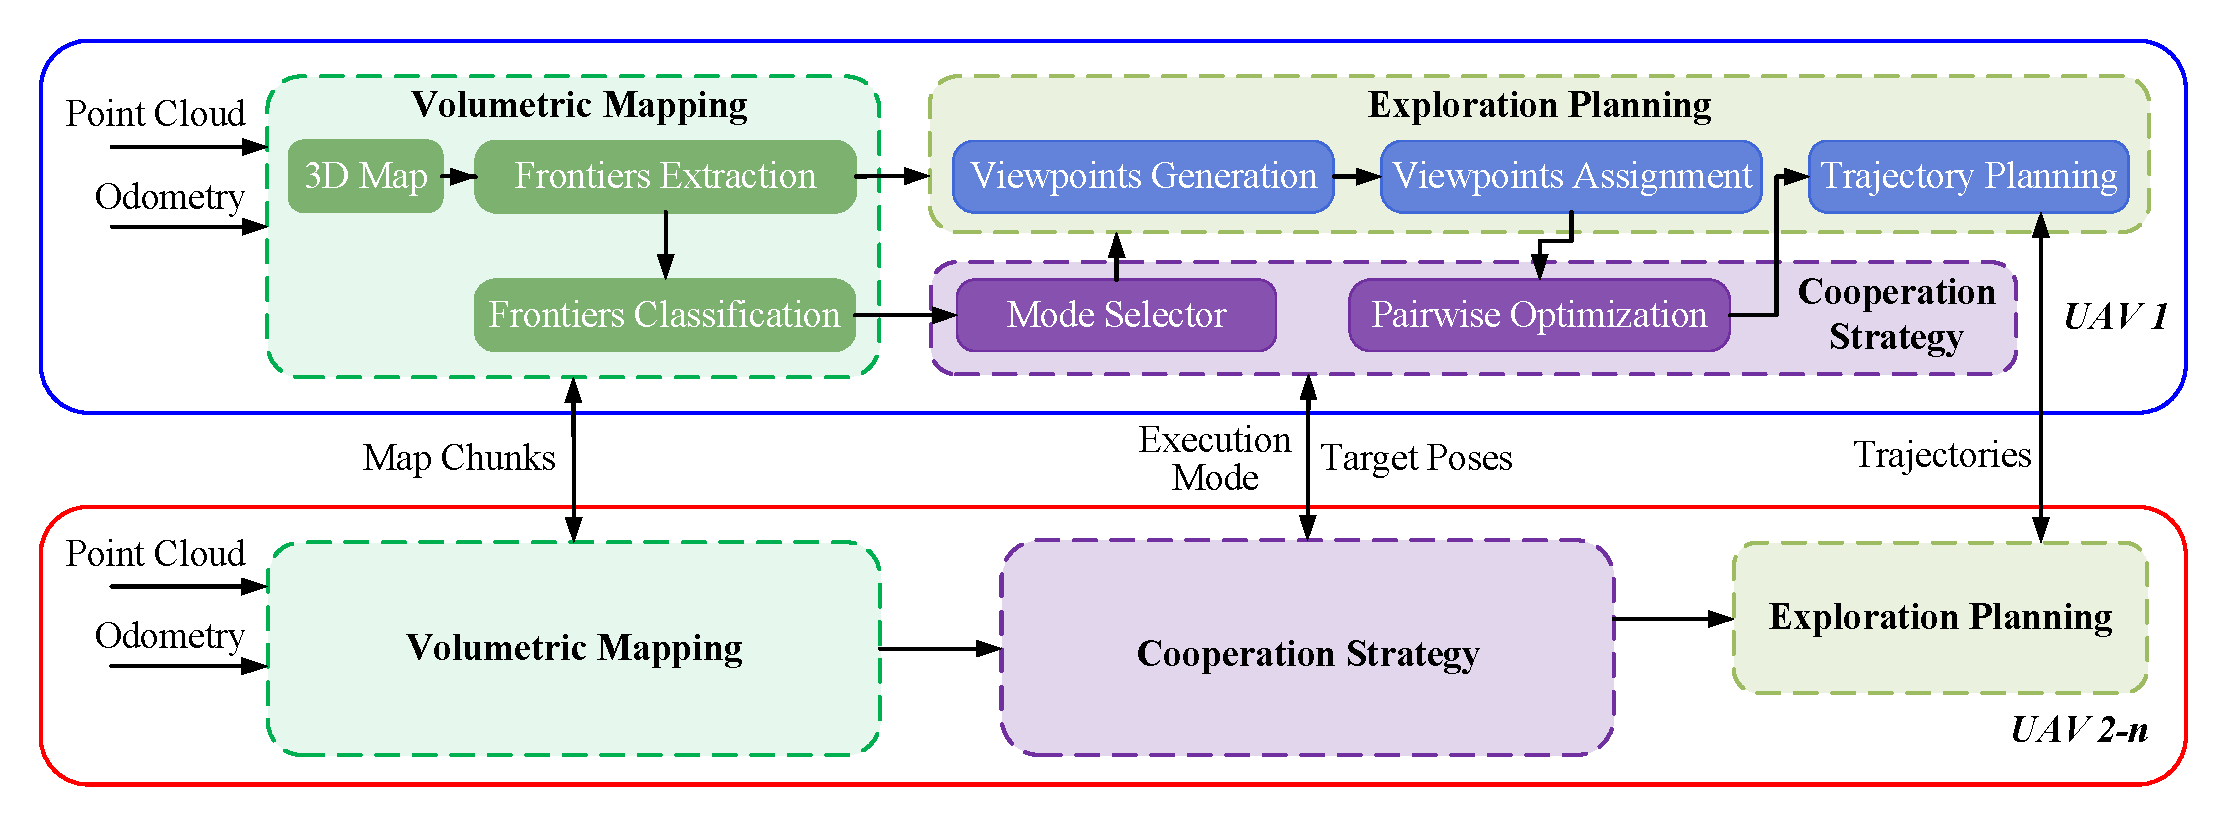
\includegraphics[width=1.98\columnwidth]{fig_overview.pdf}  
%   \vspace{-0.6cm}
  \caption{\label{fig_overview} The overview of the proposed multi-UAV cooperative exploration system. Our method's key points include low-computation-cost viewpoints generation and target viewpoints assignment. Furthermore, only the newly explored map chunks necessary for UAV motion planning are shared among UAVs.}
  % \vspace{-0.4cm}
\end{figure*}

The overall problem investigated in this work is enabling a fleet of UAVs to complete the exploration of a large, complex, and unknown environment, such as dense urban areas or forests, in the shortest possible time. We assume that each UAV is equipped with a LiDAR sensor for environmental exploration and state estimation, with a sensing range that significantly exceeds that of depth cameras. In each iteration of the exploration planning, the UAVs interact with their neighboring UAVs within the communication range, exchanging newly explored map information based on estimated relative poses, thereby making more informed decisions for the next exploration. The main difficulty of exploring large unknown environments using UAVs equipped with LiDAR lies in the high computational cost of processing the vast amount of frontier information. In fact, existing methods often generate candidate viewpoints through sampling strategies and determine the best viewpoint by calculating the number of frontier voxels covered by the sensor's FoV. It is the primary reason for the high computational cost of processing frontier information. Moreover, due to the large scale of the exploration area, issues such as UAV revisits and oscillations may still severely constrain exploration efficiency. The MAPPER proposed in this work aims to address these limitations, and the following subsections will describe its details.


\subsection{System Overview}
\label{subsec:system_overview}

The proposed pipeline for multi-UAV collaborative exploration is illustrated in Fig. \ref{fig_overview}. In this pipeline, each UAV makes exploration decisions in the decentralized set, primarily including the mapping, exploration planning, and collaboration modules. Specifically, each UAV performs incremental map construction \cite{han2019fiesta} in the mapping module by integrating its explored point cloud data with voxel information exchanged with other UAVs. After the mapping, the UAV identifies voxel cells adjacent to unknown areas in the updated map and clusters them to generate frontiers. These frontiers are then classified as either regular or island frontiers, depending on whether they have neighboring frontiers.
Next, we introduce a lightweight method proposed in this work for each frontier to perform fast viewpoint sampling, aiming to achieve the best coverage viewpoint and corresponding pose. Simultaneously, we use a dual-mode exploration strategy proposed in \cite{bartolomei2023fast} to provide the UAVs with different flight modes based on their surrounding frontiers and neighboring members. Then, the best viewpoints are allocated to UAVs by minimizing the coverage overlap of sensors' FoV and flight distance. After viewpoint allocation, we introduce pairwise interactions \cite{zhou2023racer} to optimize and determine the next target viewpoint for each UAV to visit. Finally, we employ a trajectory planner \cite{zhou2019robust} to generate feasible trajectories that enable UAVs to safely reach their respective target pose. The collaborative exploration process ends when there are no new frontiers.

\subsection{Viewpoints Generation}  
\label{subsec:generate_viewpoints}

To improve the computational efficiency of viewpoint generation, we propose an occlusion-free sector viewpoint generation strategy, illustrated in Fig. \ref{fig_gen_viewpoint}. The core idea is to quickly obtain a feasible viewpoint covering the frontier through an occlusion-free sector, thereby avoiding the computationally expensive raycasting process.
\begin{figure}[thpb]
	\centering
  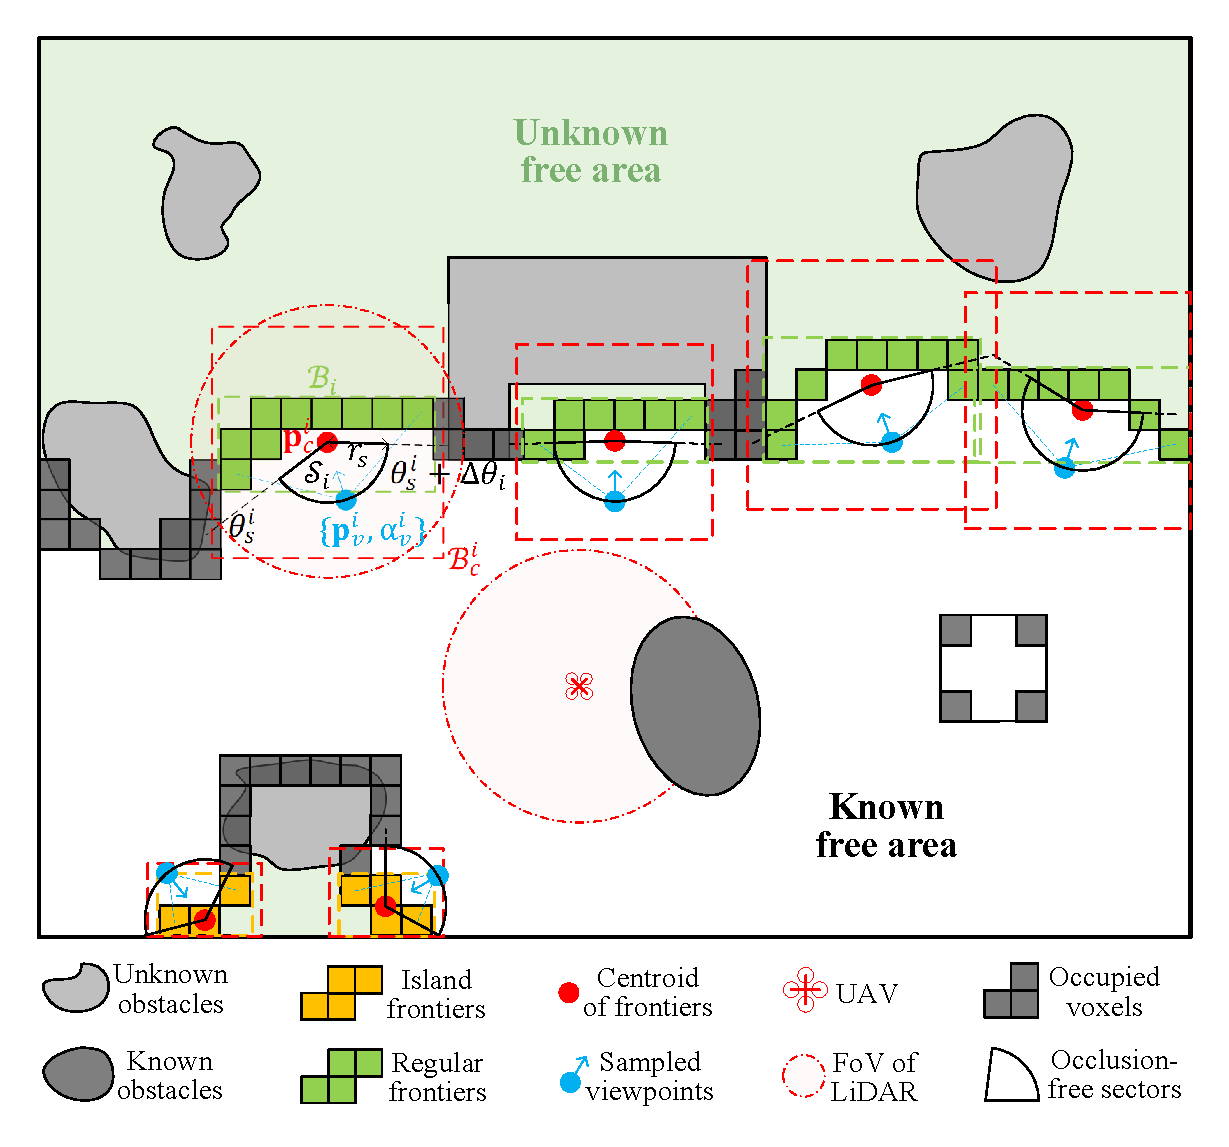
\includegraphics[width=0.98\columnwidth]{fig_gen_viewpoint.pdf}  
%   \vspace{-0.6cm}
  \caption{\label{fig_gen_viewpoint} The geometric illustration of the proposed occlusion-free sector viewpoint sampling strategy.}
  % \vspace{-0.4cm}
\end{figure}

We denote the frontiers set in the environment as \( \boldsymbol{\mathcal{F}}\). Then, let $\mathcal{F}_i \in \boldsymbol{\mathcal{F}}$ represent a frontier whose information structure includes the label $\mathcal{L}_i$ ((marking regular frontiers and island frontiers)), the cluster $\mathcal{C}_i$ of unoccupied voxel cells adjacent to the unknown region, the average position $\mathbf{p}_c^i \in \mathbb{R}^3$ of the cluster $\mathcal{C}_i$, and the axis-aligned bounding box (AABB) $\mathcal{B}_i$ of the cluster $\mathcal{C}_i$. Additionally, we define another AABB $\mathcal{B}_c^i$, centered at $\mathbf{p}_c^i$, with all its edge lengths equal to the diagonal length (Euclidean distance) of $\mathcal{B}_i$. 
%The minimum and maximum points of \(\mathcal{B}_c^i\) are \(\mathbf{p}_{\min}^i\) and \(\mathbf{p}_{\max}^i\), respectively.
Next, we define the occlusion-free sector of $\mathcal{F}_i$ as follows:
\begin{equation}
  \label{Equation1}
  \begin{aligned}
    \mathcal{S}_i = \left\{ \mathbf{p} \mid \| \mathbf{p} - \mathbf{p}_c^i \| \leq r_s, \, \theta_s^i \leq \theta(\mathbf{p} - \mathbf{p}_c^i) \leq \theta_s^i+\Delta\theta_i \right\},
  \end{aligned}
\end{equation}
where \( \mathcal{S}_i \) is the occlusion-free sector around the frontier \( \mathcal{F}_i \), \( \mathbf{p} \in \mathbb{R}^3\) is any point in space, \( r_s \) is the radial distance from the center $\mathbf{p}_c^i$ to the arc boundary of the sector \( \mathcal{S}_i \), \( \theta_s^i \) is the starting angle of the sector, \( \Delta\theta_i \) is the angular span of \( \mathcal{S}_i \), and \( \theta(\mathbf{p} - \mathbf{p}_c^i) \) indicates the angle of the vector $\mathbf{p} - \mathbf{p}_c^i$ relative to the X-axis. It should be noted that the value of \(r_s\) is determined by the sampling radius, and the sector \( \mathcal{S}_i \) does not exceed the bounding box \(\mathcal{B}_c^i\).

We further present how to calculate the occlusion-free sector's \( \theta_s \) and \( \Delta\theta \). First, we calculate the angle of the vector from \(\mathbf{p}_c^i\) to any occupied or unknown voxel within \(\mathcal{B}_c^i\) relative to the X-axis using Equation (\ref{Equation2}), which generates the set of angles \(\Theta_i = \{\theta_i^1, \theta_i^2, \dots, \theta_i^{k}\}\):
\begin{equation}
  \label{Equation2}
  \begin{aligned}
    \theta_i^j = \theta(\mathbf{p}_{ou}^j - \mathbf{p}_c^i), \quad j \in \{1, 2, ..., k\},
  \end{aligned}
\end{equation}
where $\mathbf{p}_{\min}^i \leq \mathbf{p}_{ou}^j \leq \mathbf{p}_{\max}^i$, and \(k\) is the number of occupied and unknown voxels within \(\mathcal{B}_c^i\).
Subsequently, we sort the angle values in $\Theta_i$ in increasing order to obtain the ordered set of angles $\Theta_{\text{sorted}}^i = \{ \theta_i^{(1)}, \theta_i^{(2)}, \dots, \theta_i^{(k)} \}$. 
By identifying the largest difference between adjacent angles, we obtain $\theta_s^i$ and $\Delta\theta_i$ as defined in Equation (\ref{Equation1}). 
We obtain $\theta_s^i$ and $\Delta\theta_i$ as defined in Equation (\ref{Equation1}) by identifying the largest difference between adjacent angles.
Notably, by considering both the occupied and unknown voxels within \( \mathcal{B}_c^i \), we ensure that the obtained sector lies within the known region. The mathematical expression is summarized as follows:
\begin{equation}
  \label{Equation3}
  \begin{aligned}
    j_{\max} = \arg\max_j \Delta \theta_i^{(j)},\quad j \in \{1, 2, ..., k\},
  \end{aligned}
\end{equation}
\begin{equation}
  \label{Equation4}
  \begin{aligned}
    \theta_s^i = \theta_i^{(j_{\max})}, \quad \Delta\theta_i = \Delta \theta_i^{(j_{\max})},
  \end{aligned}
\end{equation}
where $\Delta \theta_i^{(j)}$ is the difference between two adjacent angles in $\Theta_{\text{sorted}}^i$, which can be calculated using the following formulation:
\begin{equation}
	\label{Equation5}
	\Delta \theta_i^{(j)}=
	\begin{cases} 
		\theta_i^{(1)} - \theta_i^{(k)}, & \text{if } j=k \\
		\theta_i^{(j+1)} - \theta_i^{(j)}, & \text{otherwise}.
	\end{cases}
\end{equation}


After computing the occlusion-free sector \(\mathcal{S}_i\) around a frontier \(\mathcal{F}_i\), intuitively, among the candidate viewpoints sampled along the arc boundary of the sector, the viewpoint located at the midpoint of the arc generally provides the most extensive coverage. Therefore, we select the midpoint of the arc boundary as the most feasible viewpoint $\mathbf{p}_{v}^i$ and set its orientation angle $\alpha_{v}^i$ as the direction from this viewpoint to the sector's center \(\mathbf{p}_c^i\), as illustrated in Fig. \ref{fig_gen_viewpoint}. The pose $\{\mathbf{p}_{v}^i, \alpha_{v}^i\}$ can be computed using the following formulation:
\begin{equation}
	\label{Equation6}
		\begin{cases} 
      \mathbf{p}_{v}^i = [\cos(\theta_{mid}^i), \sin(\theta_{mid}^i), z_{c}^i], \\
      \alpha_{v}^i = \theta(\mathbf{p}_{v}^i - \mathbf{p}_c^i), 
	\end{cases}
\end{equation}
where \(z_c^i\) is the \(z\)-coordinate of \(\mathbf{p}_c^i\), and \(\theta_{mid}^i = \theta_{s}^i + 0.5\Delta\theta_i\).
It should be noted that the viewpoint calculated by Equation (\ref{Equation6}) is not the optimal one but rather a trade-off solution aimed at improving the computational efficiency of viewpoint sampling while ensuring sampling quality. Since the bounding box \(\mathcal{B}_c^i\) completely encloses the frontier cluster \(\mathcal{C}_i\) and their neighboring voxels, when the angular span $\Delta\theta_i$ of the occlusion-free sector \(\mathcal{S}_i\) exceeds $\Delta\theta_{min}$, the viewpoint $\mathbf{p}_{v}^i$ obtained through the occlusion-free sector can ensure a high coverage for the UAV. Empirically, we set \(\Delta\theta_{min}\) to \(\frac{\pi}{6}\). Meanwhile, when the angular span $\Delta\theta_i$ is smaller, we resort to the sampling method used in \cite{zhou2023racer} to ensure the completeness of viewpoint sampling. In most cases, the proposed occlusion-free sector method can computer a feasible viewpoint, thus improving the efficient computation of viewpoint sampling.

\subsection{Viewpoint Assignment and Pairwise Optimization}
\label{subsec:viewpoint_assignment}

In viewpoint assignment, we aim to ensure that each drone moves towards the target viewpoint with the minimum cost while minimizing the overlapping areas of the perception range between drones. To avoid drones revisiting the frontier of unexplored islands missed due to sensor occlusion caused by obstacles, we introduce the dual-mode exploration strategy proposed in \cite{bartolomei2023fast}: the Explorer mode and the Collector mode. In the Explorer mode, drones prioritize exploring larger unknown areas with cautious movements. Since most of the environment is unknown, drones choose a cautious flying speed for safety in this mode. In contrast, in the Collector mode, drones mainly explore the unexplored island areas (such as the unknown areas around the Island frontiers in Fig. \ref{fig_assign}). As most of the environment has already been explored and mapped, drones can adopt a more aggressive flying speed to cover the island areas more quickly. Importantly, as the sensor's perception range increases, the pipeline in \cite{bartolomei2023fast} encounters significant bottlenecks, such as the frequent request of the time-consuming A* algorithm to compute path costs and the tendency for allocated areas of interest to have significant overlaps in the perception range between drones. The method proposed in this paper effectively addresses these limitations. 

\begin{figure}[thpb]
	\centering
  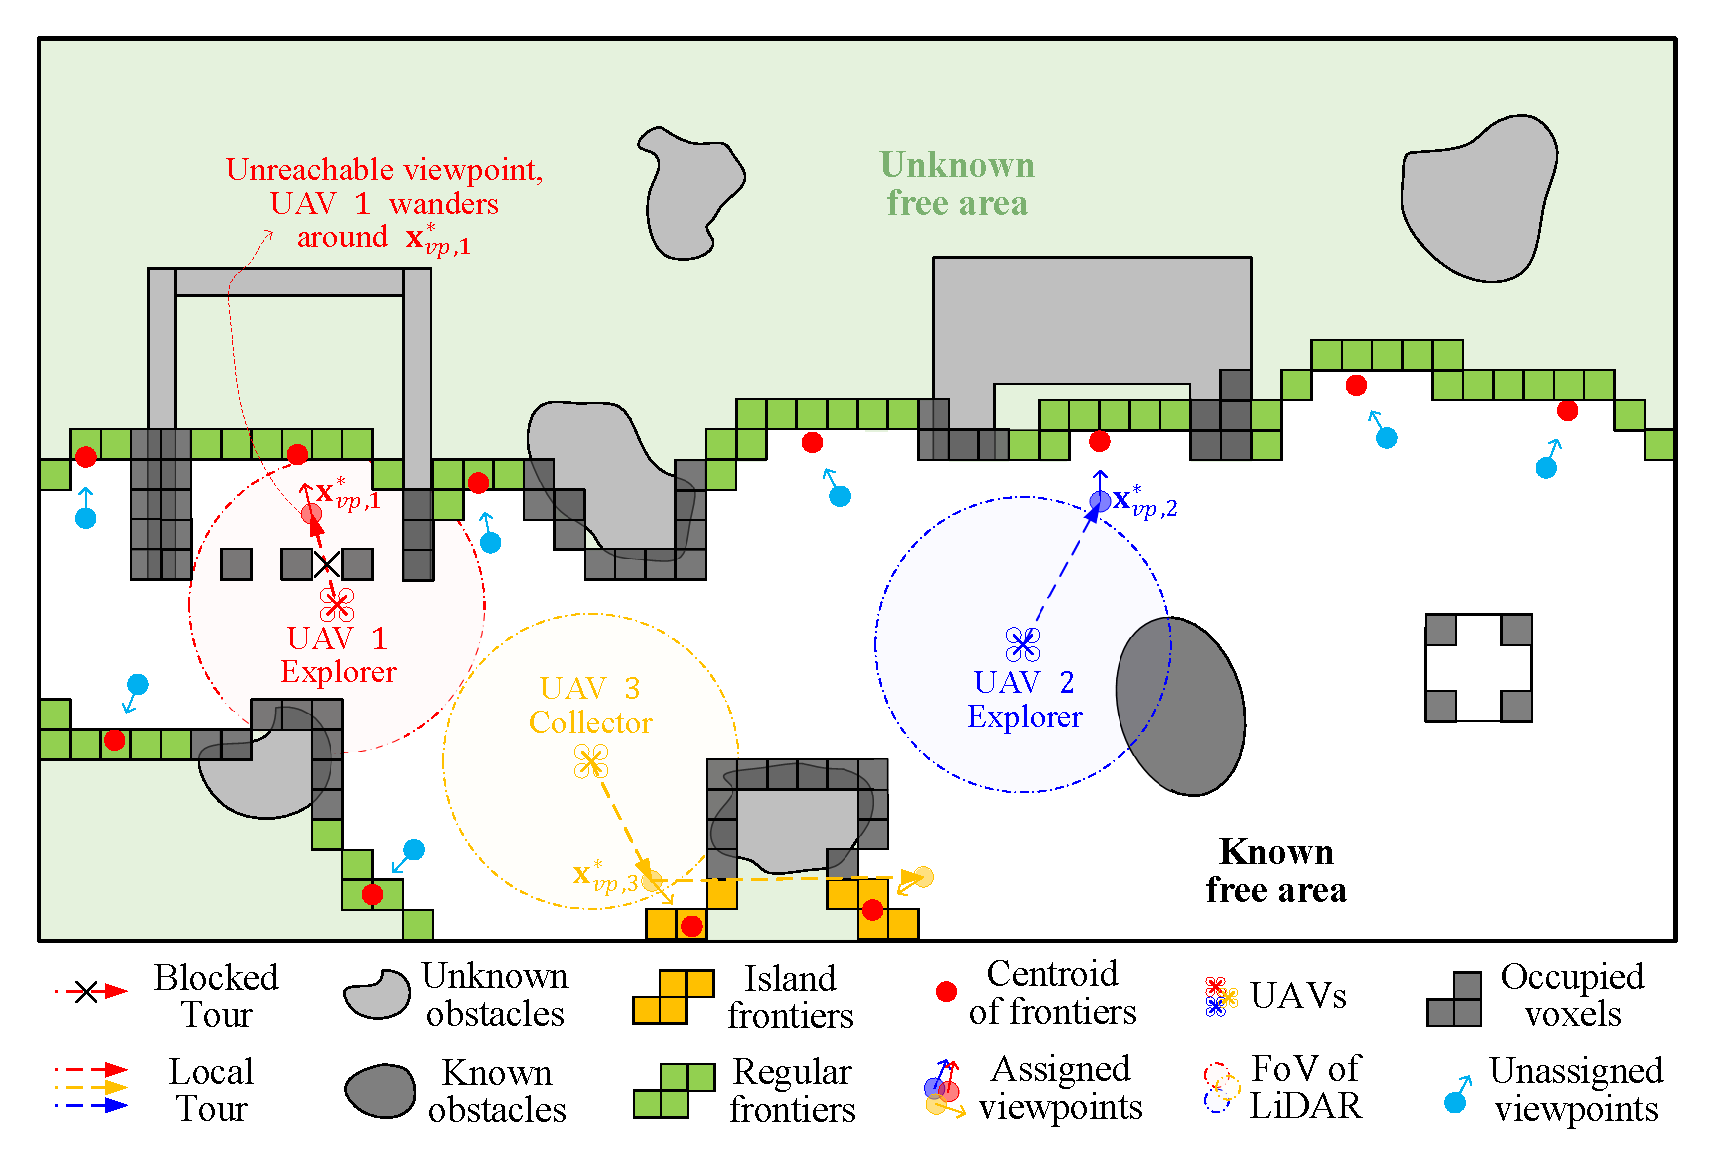
\includegraphics[width=0.98\columnwidth]{fig_assign.pdf}  
%   \vspace{-0.6cm}
  \caption{\label{fig_assign} The geometric illustration of viewpoint assignment in an exploration planning iteration, including the results of viewpoint assignment and cases of unreachable viewpoints.}
  % \vspace{-0.4cm}
\end{figure}

Now, we present the proposed viewpoint assignment method for drones in the Explorer mode. First, we define the cost \( J_C \) for UAV \( i \) to fly from its current state \( \mathbf{x}_U^i = \{ \mathbf{p}_U^i, \alpha_U^i \} \) to a target viewpoint \( \mathbf{x}_{vp} = \{ \mathbf{p}_v, \alpha_v \} \), where $\mathbf{p}_* \in \mathbb{R}^3$ is the position and $\alpha_* \in \mathbb{R}$ the orientation. The expression for the cost \( J_C \) is as fo
llows:
\begin{equation}
  \label{eq_assign1}
  \begin{aligned}
      J_{C}(\mathbf{x}_U^i, \mathcal{X}_U^i, \mathcal{X}_G^i, \mathbf{x}_{vp}) = \omega_D^e J_D + \omega_V^e J_V + \omega_O J_O,
  \end{aligned}
\end{equation}
where \( J_D \) is the path length between the current position \( \mathbf{p}_U^i \) of UAV \( i \) and the target viewpoint position \( \mathbf{p}_v \), which is calculated using the A* algorithm; \( J_V \) refers to the cost of changing the direction of travel; \( J_O \) is the cost of overlapping perception ranges between UAVs; the \( \omega_D^e \), \( \omega_V^e \), and \( \omega_O \) are constant weights; \( \mathcal{X}_U^i \) and \( \mathcal{X}_G^i \) are the current positions and target positions of all neighboring UAVs for UAV $i$, respectively.
In order to improve the motion consistency of UAV $i$, we prioritize the viewpoint in front of the UAV's heading and define the frontier voxel cluster in front of the UAV's heading as \( \mathcal{C}_f \subseteq \mathcal{C} \). Thus, we define the formulation for \( J_V \) as follows:
\begin{equation}
  \label{eq_assign2}
  J_V(\mathbf{x}_U^i, \mathbf{x}_{vp})=
	\begin{cases} 
		1 - ( 
      \frac{\mathbf{v}_U^i}{\|\mathbf{v}_U^i\|} \cdot
      \frac{\mathbf{p}_{v} - \mathbf{p}_U^i}{\|\mathbf{p}_{v} - \mathbf{p}_U^i\|}
      ), & \text{if } \mathcal{C}_f=\emptyset \\
      \arccos( 
      \frac{\mathbf{v}_U^i}{\|\mathbf{v}_U^i\|} \cdot
      \frac{\mathbf{p}_{v} - \mathbf{p}_U^i}{\|\mathbf{p}_{v} - \mathbf{p}_U^i\|}
      ), & \text{otherwise},
	\end{cases}
\end{equation}
where \(\mathbf{v}_U^i\) represents the current velocity of UAV \(i\), note that when \(\mathcal{C}_f\) is not an empty set, we only consider the viewpoints corresponding to \(\mathcal{C}_f\). 
In addition, to improve computational efficiency and minimize the overlap of perception ranges between UAVs, we directly determine the \(J_O\) by the distances between the target viewpoint \(\mathbf{x}_{vp}\) and all positions in \(\mathcal{X}_U^i\) and \(\mathcal{X}_G^i\). If all distances are greater than $R_{sense}$, the value of \(J_O\) is 0; otherwise, the value of \(J_O\) is infinity. Empirically, we set $R_{sense}$ to half of the sensor's maximum sensing distance.
Finally, the best target pose \(\mathbf{x}_{vp, i}^*\) for UAV $i$ with the minimum cost is selected from the viewpoints set $\mathcal{X}_{vp}$ corresponding to all frontiers. The expression is as follows:
\begin{equation}
  \label{eq_assign3}
  \begin{aligned}
    \mathbf{x}_{vp, i}^*= \arg\min_{\forall \mathbf{x}_{vp} \in \mathcal{X}_{vp}} J_C(\mathbf{x}_U^i, \mathcal{X}_U^i, \mathcal{X}_G^i, \mathbf{x}_{vp}).
  \end{aligned}
\end{equation}

Next, we describe the viewpoint allocation strategy for UAVs in the Collector mode. The objective is to clear as many unexplored isolated areas near the UAV as possible, avoiding significant detours by other UAVs to revisit these areas. To achieve this, we use the Asymmetric Traveling Salesman Problem (ATSP) \cite{zhou2023racer} to plan the UAV's path for clearing these isolated areas.
First, we prioritize determining whether the viewpoints covering the isolated areas are within the current perception range of other UAVs or the target viewpoints of other UAVs. If so, these isolated areas are excluded from the current viewpoint allocation to reduce the overlapping perception areas between UAVs. For the remaining \(N_I\) isolated regions that are not within the above perception range, we design a cost matrix \(\mathbf{M} \in \mathbb{R}^{(N_I+1)\times(N_I+1)}\) for the UAV to clear these isolated regions. The expression of this matrix is as follows: 
\begin{equation}
	\label{eq_assign4}
		\begin{cases} 
      \mathbf{M}(i, j) = \omega_D^c J_D(\mathbf{x}_{vp}^i, \mathbf{x}_{vp}^j) + \omega_V^c J_V(\mathbf{x}_{vp}^i, \mathbf{x}_{vp}^j), \\
      \mathbf{M}(0, i) = \omega_D^c J_D(\mathbf{x}_U, \mathbf{x}_{vp}^i) + \omega_V^c J_V(\mathbf{x}_U, \mathbf{x}_{vp}^i), 
	\end{cases}
\end{equation}
where the definitions of \( J_D \) and \( J_V \) are consistent with those in the Collector mode, the terms \( \omega_D^c \) and \( \omega_V^c \) are constant weights, \( \mathbf{x}_{vp}^i \) and \( \mathbf{x}_{vp}^j \) is the poses of two target viewpoints, and \( \mathbf{x}_U \) is the current pose of the UAV.

It is important to note that during the viewpoint assignment process, to reduce computational costs, the A* algorithm is typically employed in coarse search (i.e., using a larger voxel resolution) to compute the path length \( J_D \). In subsequent trajectory planning, obstacles may block the UAV’s path, preventing it from reaching the assigned target viewpoint. As illustrated in Fig. \ref{fig_assign}, UAV $1$ wanders around the assigned target viewpoint, which is unreachable. It can severely impact the overall exploration efficiency. 
To address this issue, during each exploration planning iteration, we check whether the UAV's current position is too close to its previous position during the last iteration. If so, we increment \( N_{\text{near}} \); otherwise, we reset \( N_{\text{near}} \) to zero. When \( N_{\text{near}} \) exceeds a predefined threshold \( N_{\text{near}}^{\max} \), we use the viewpoint assignment strategy in the Explorer mode to change the UAV's target viewpoint forcibly. This mechanism prevents a UAV from becoming stuck and wandering around an unreachable viewpoint, improving the overall exploration efficiency of the UAV team.
Additionally, after the viewpoint assignment, we use the pairwise interaction \cite{zhou2023racer} to swap the target viewpoints between two UAVs. If the swap results in a lower overall cost, the new assignment will be adopted; otherwise, the original assignment will be retained. The pairwise interaction optimization of viewpoint assignment further ensures the rationality of the viewpoint allocation.


\section{Experimental Evaluation}
\label{sec:experiments}

\begin{figure*}[thpb]
  \centering
  \subfigtopskip=0pt
  \subfigbottomskip=2pt
  \subfigcapskip=-3pt 
  \subfigure[]{
\includegraphics[width=0.61\columnwidth]{building.jpg}}   
  \subfigure[]{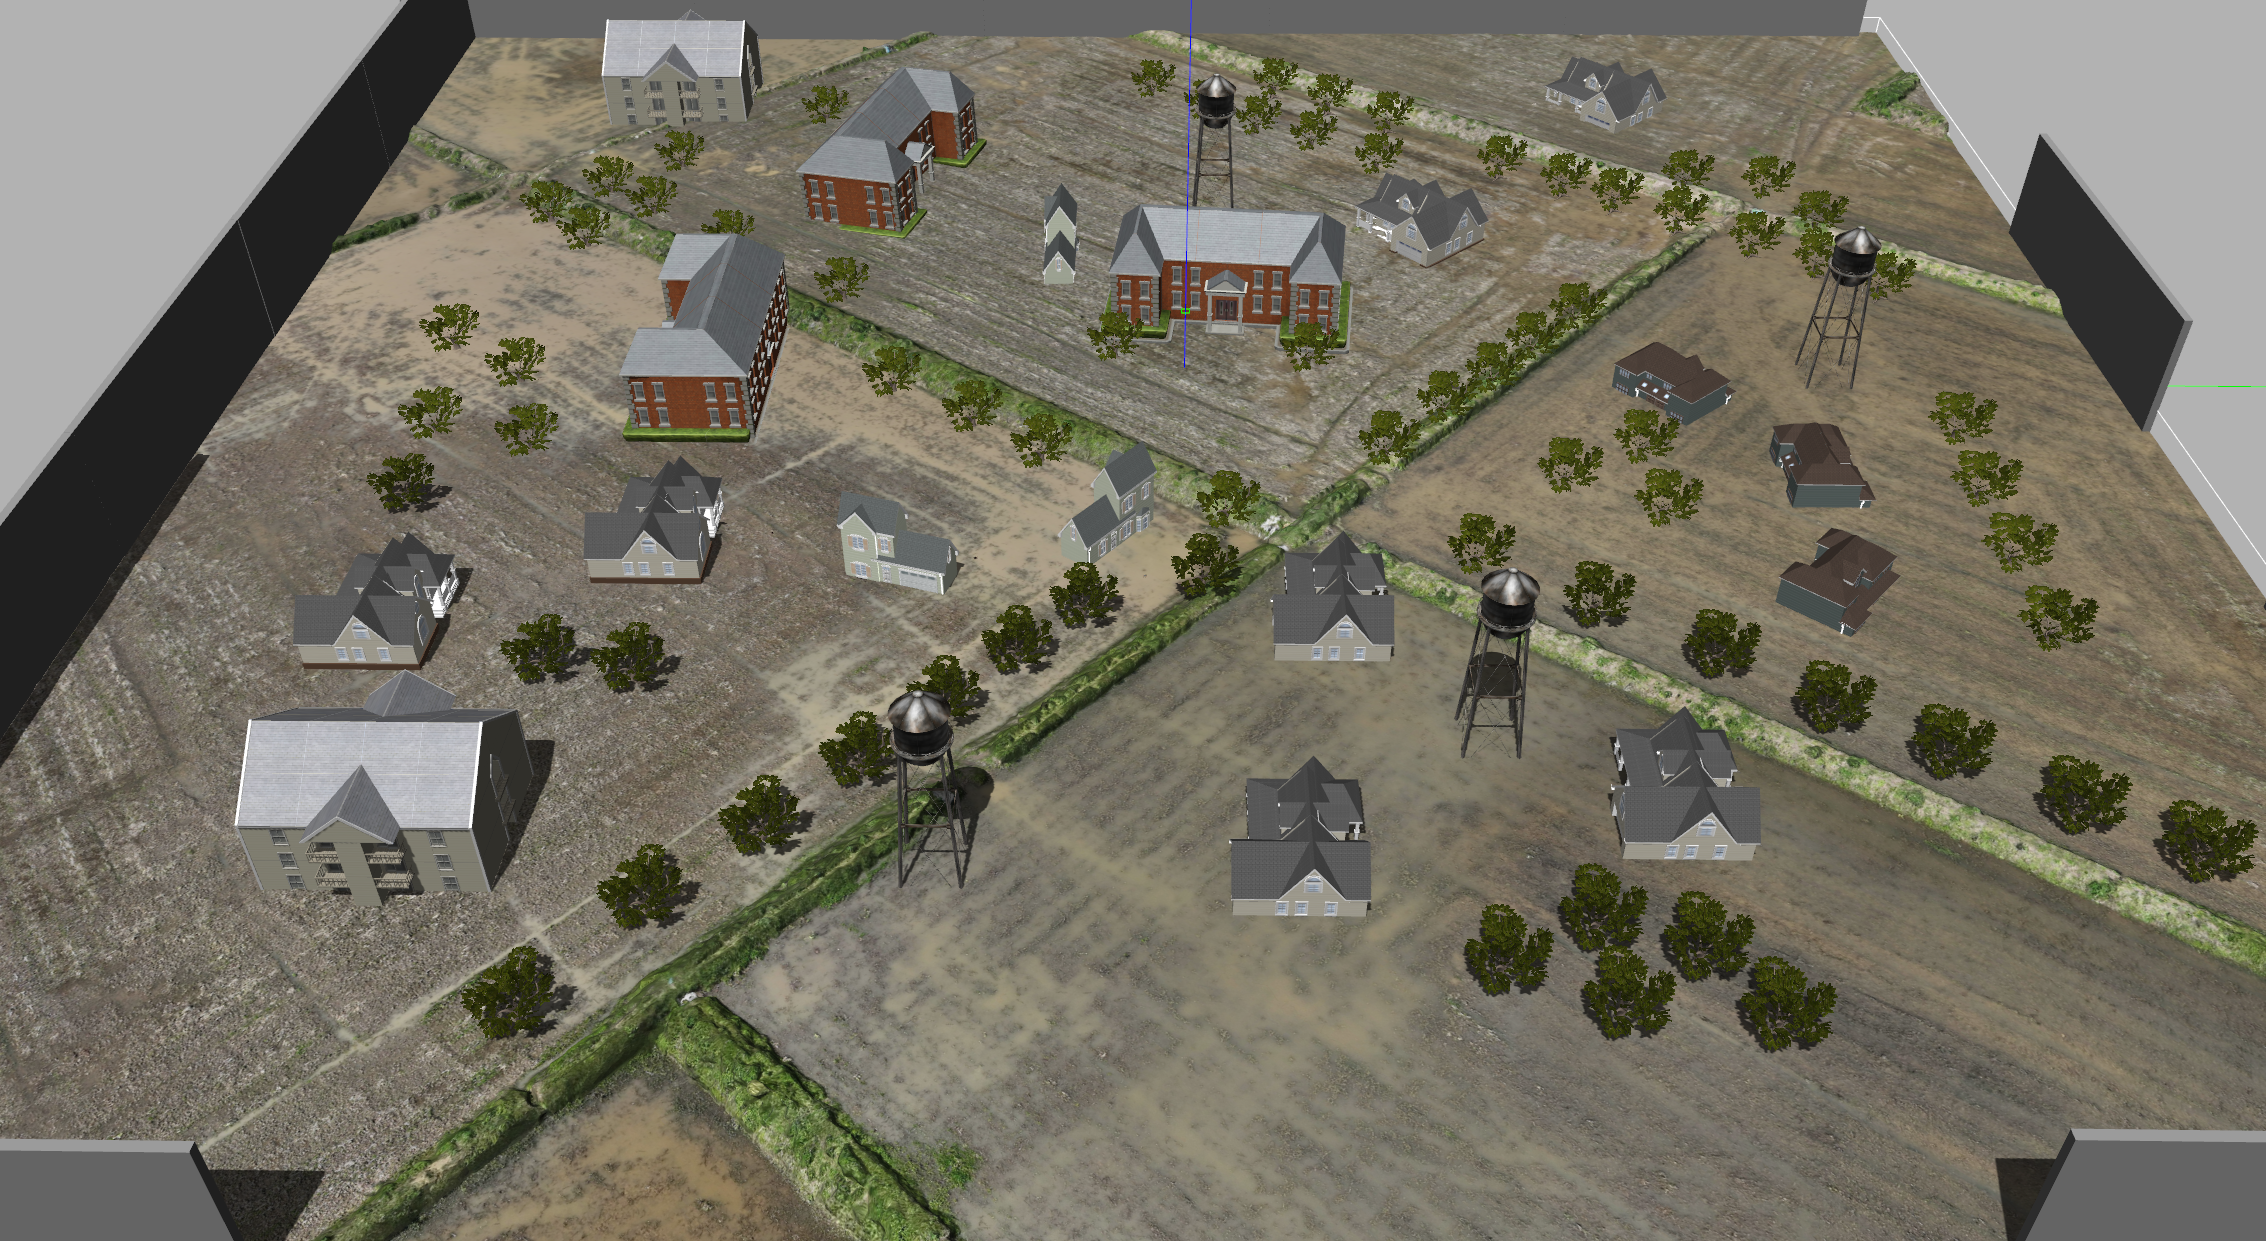
\includegraphics[width=0.607\columnwidth]{village.jpg}}   
  \subfigure[]{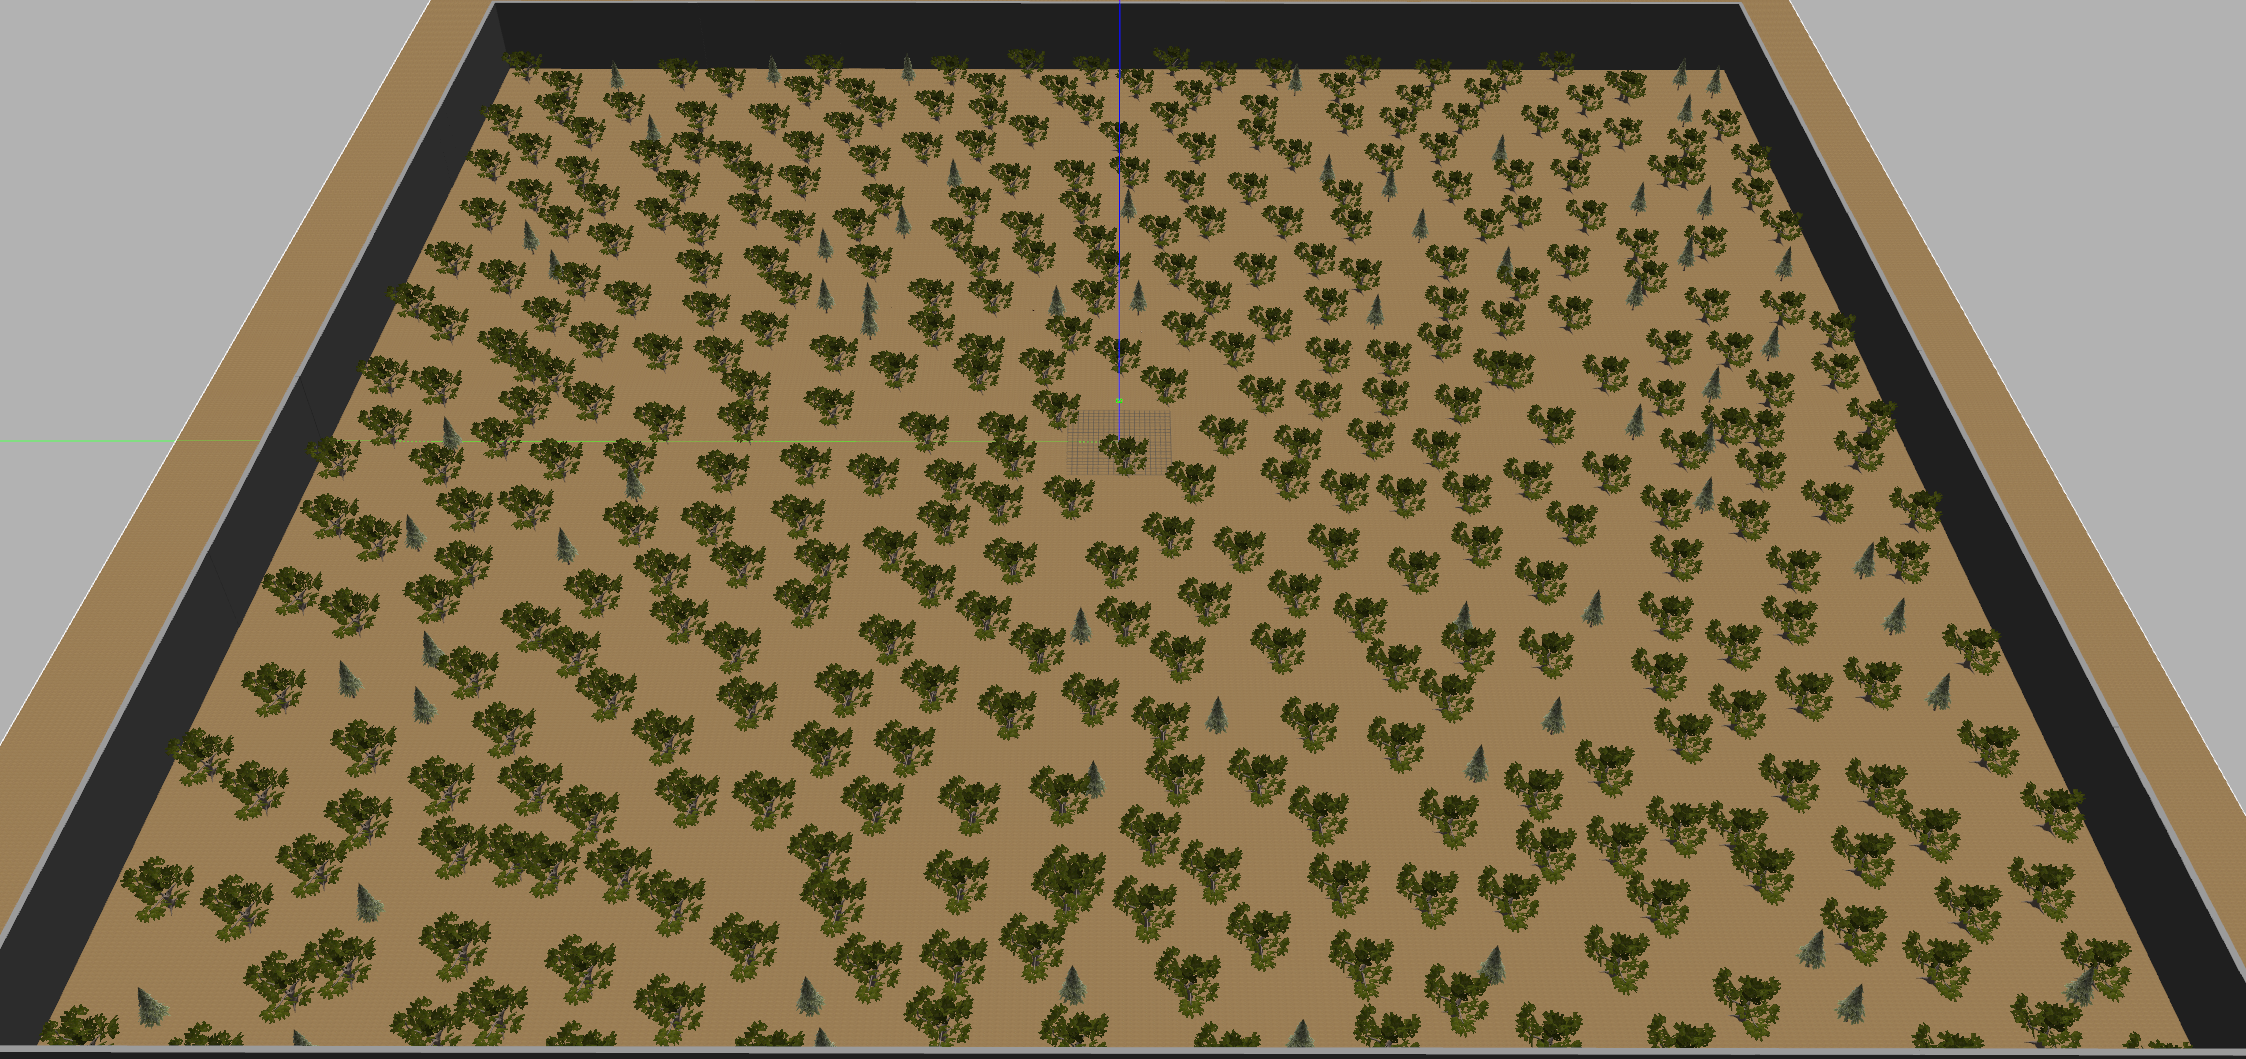
\includegraphics[width=0.707\columnwidth]{forest.jpg}}  

  \subfigure[]{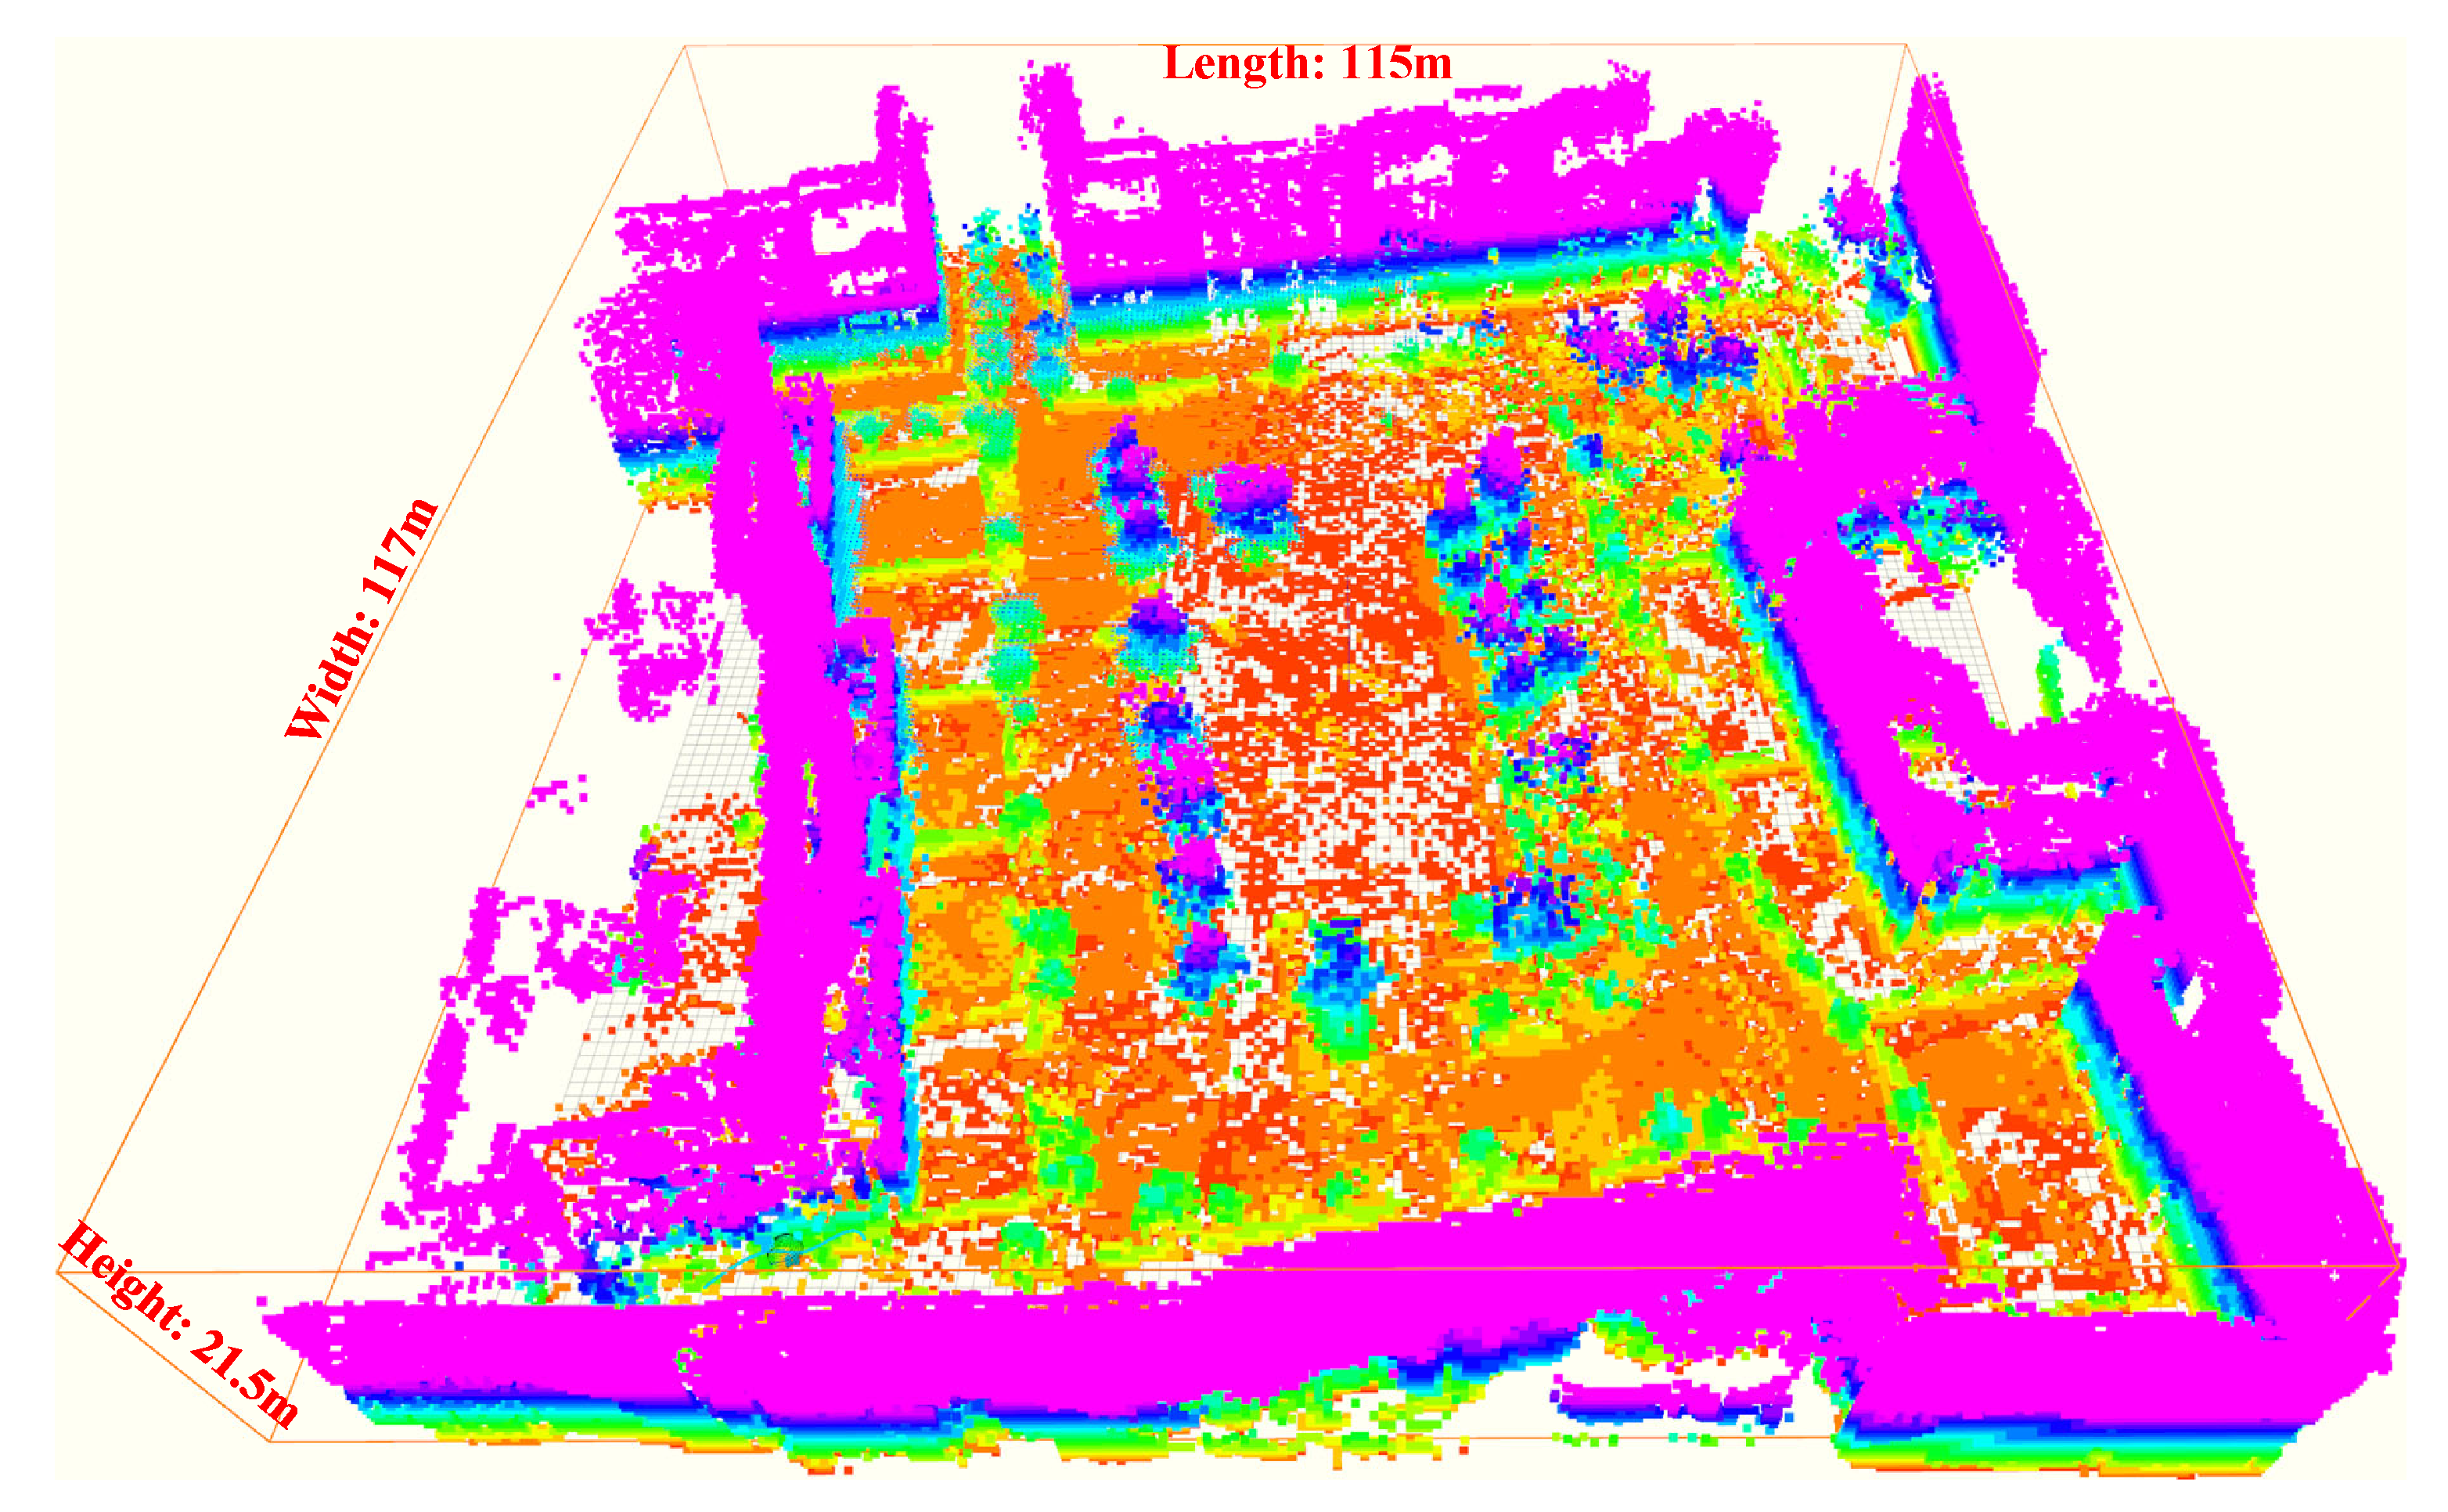
\includegraphics[width=0.6\columnwidth]{s1.pdf}}   
  \subfigure[]{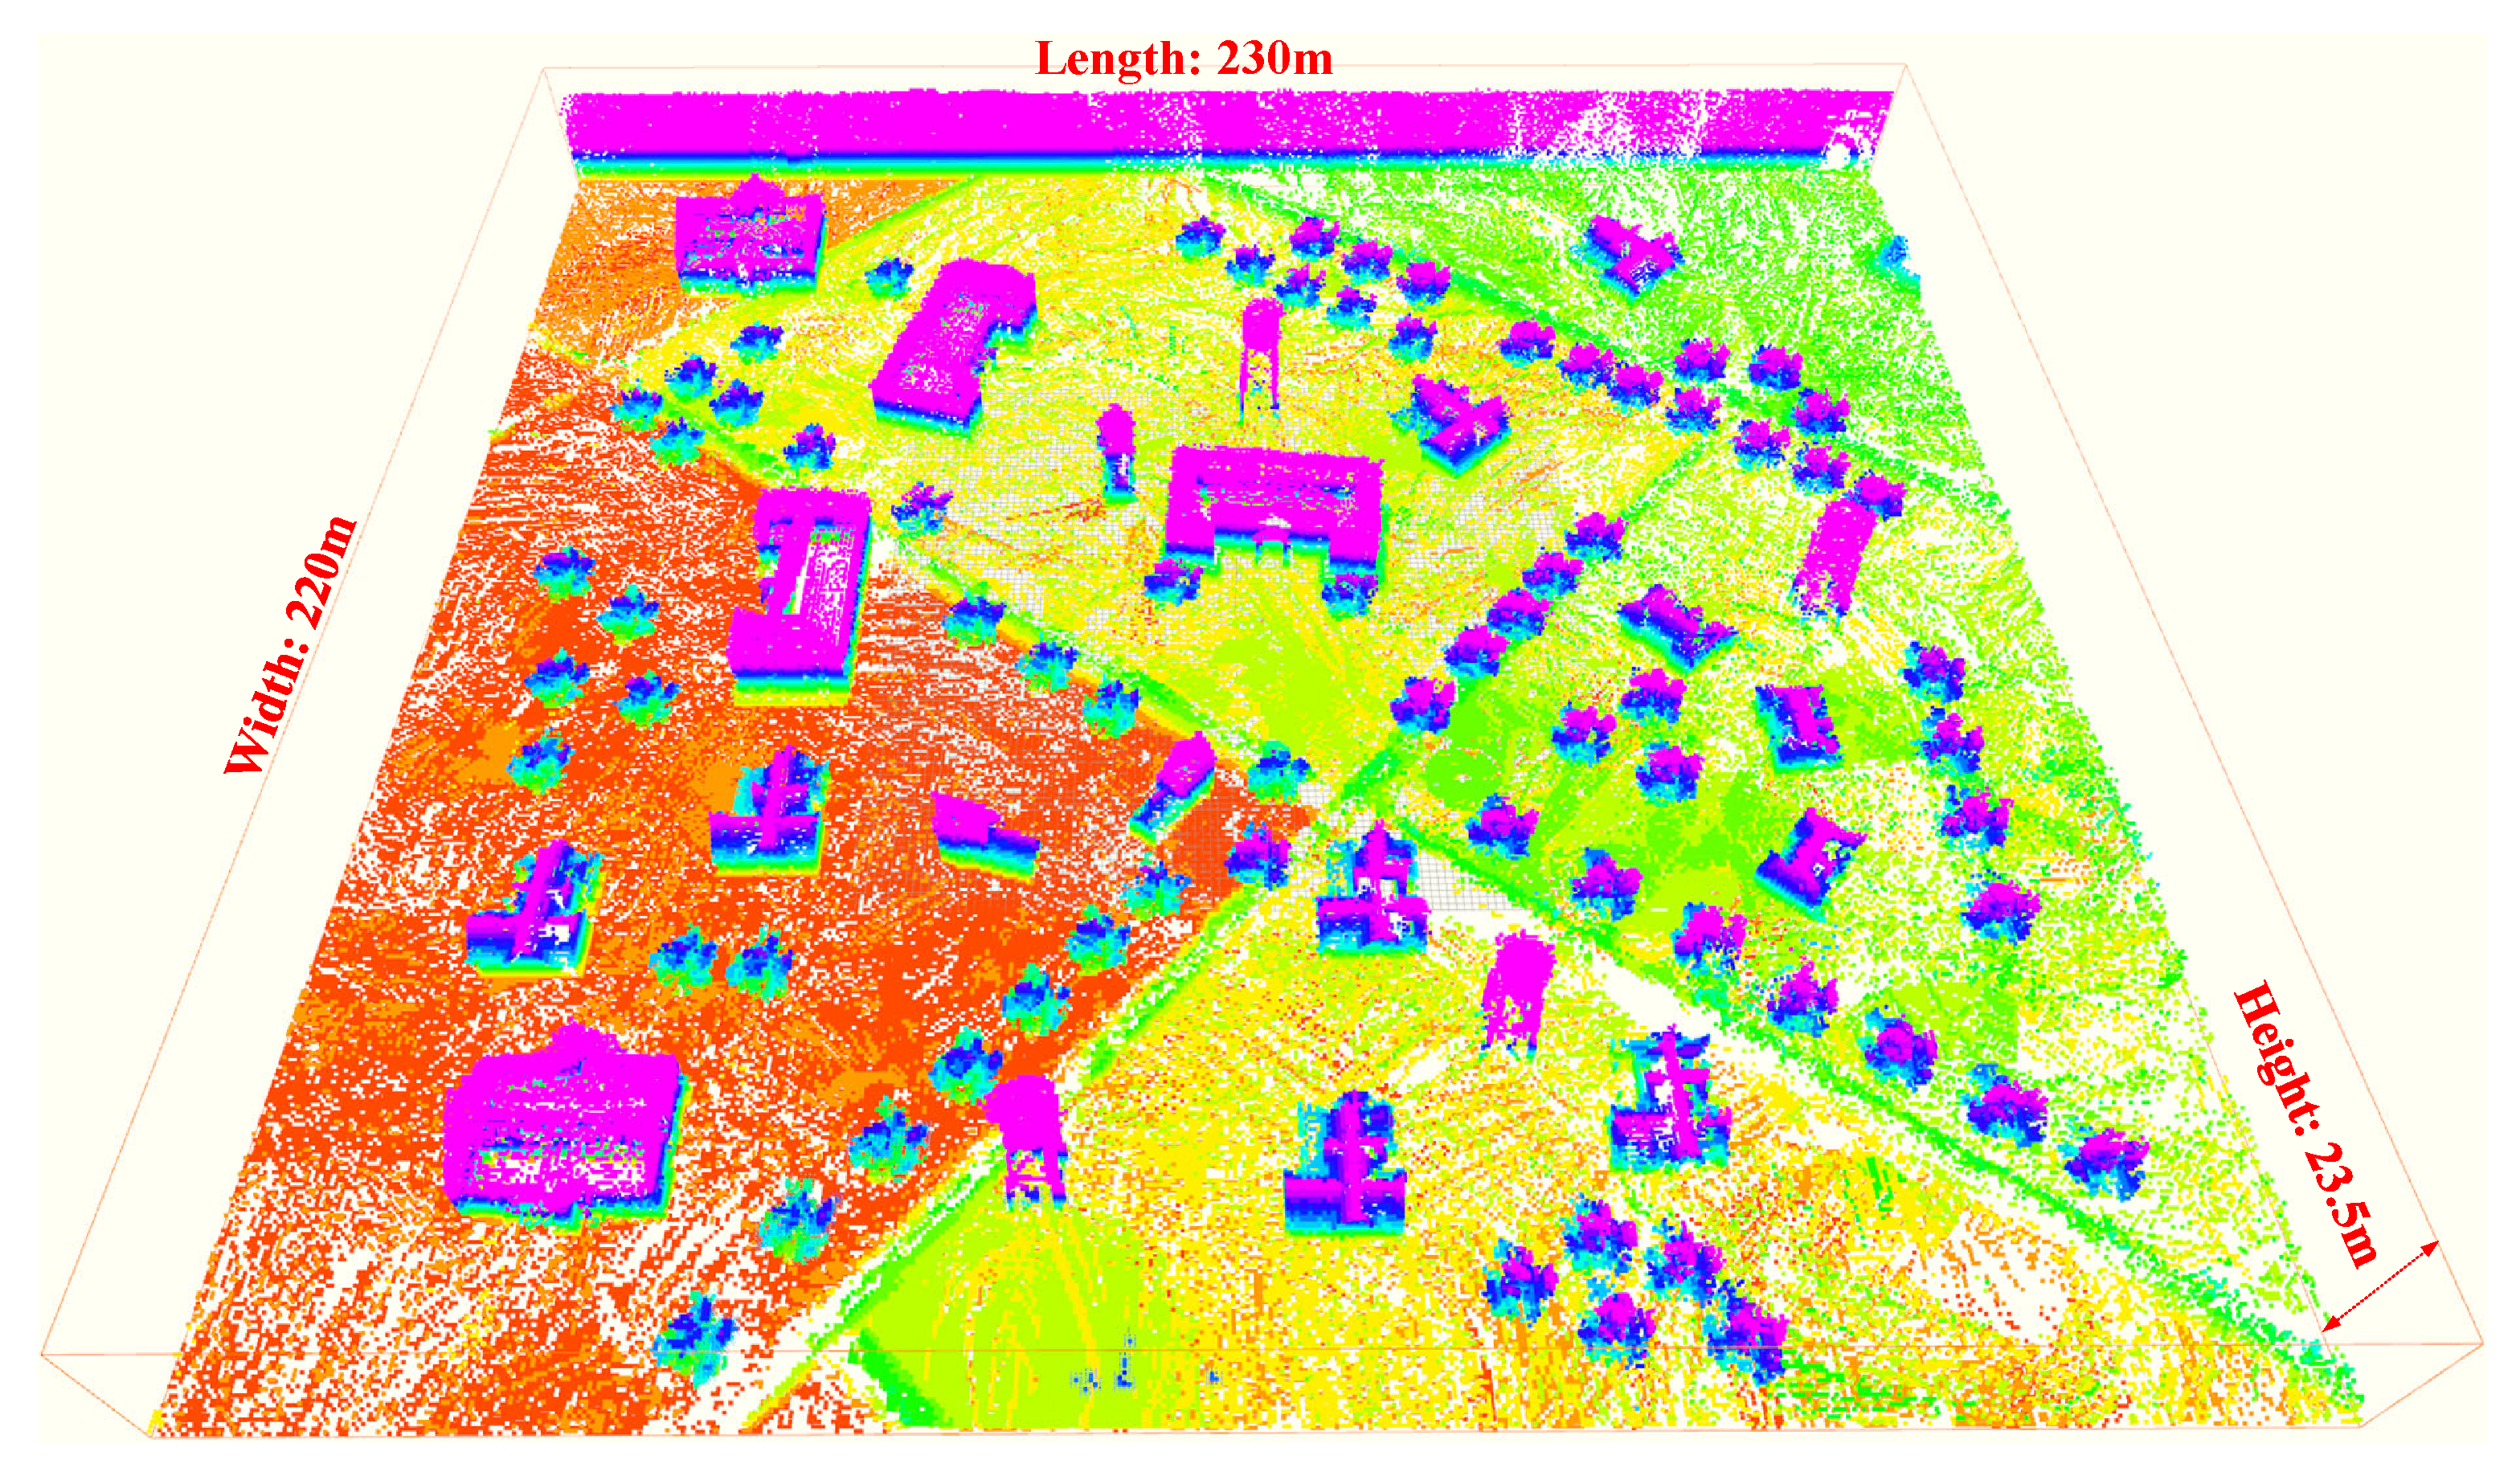
\includegraphics[width=0.64\columnwidth]{s2.pdf}}   
  \subfigure[]{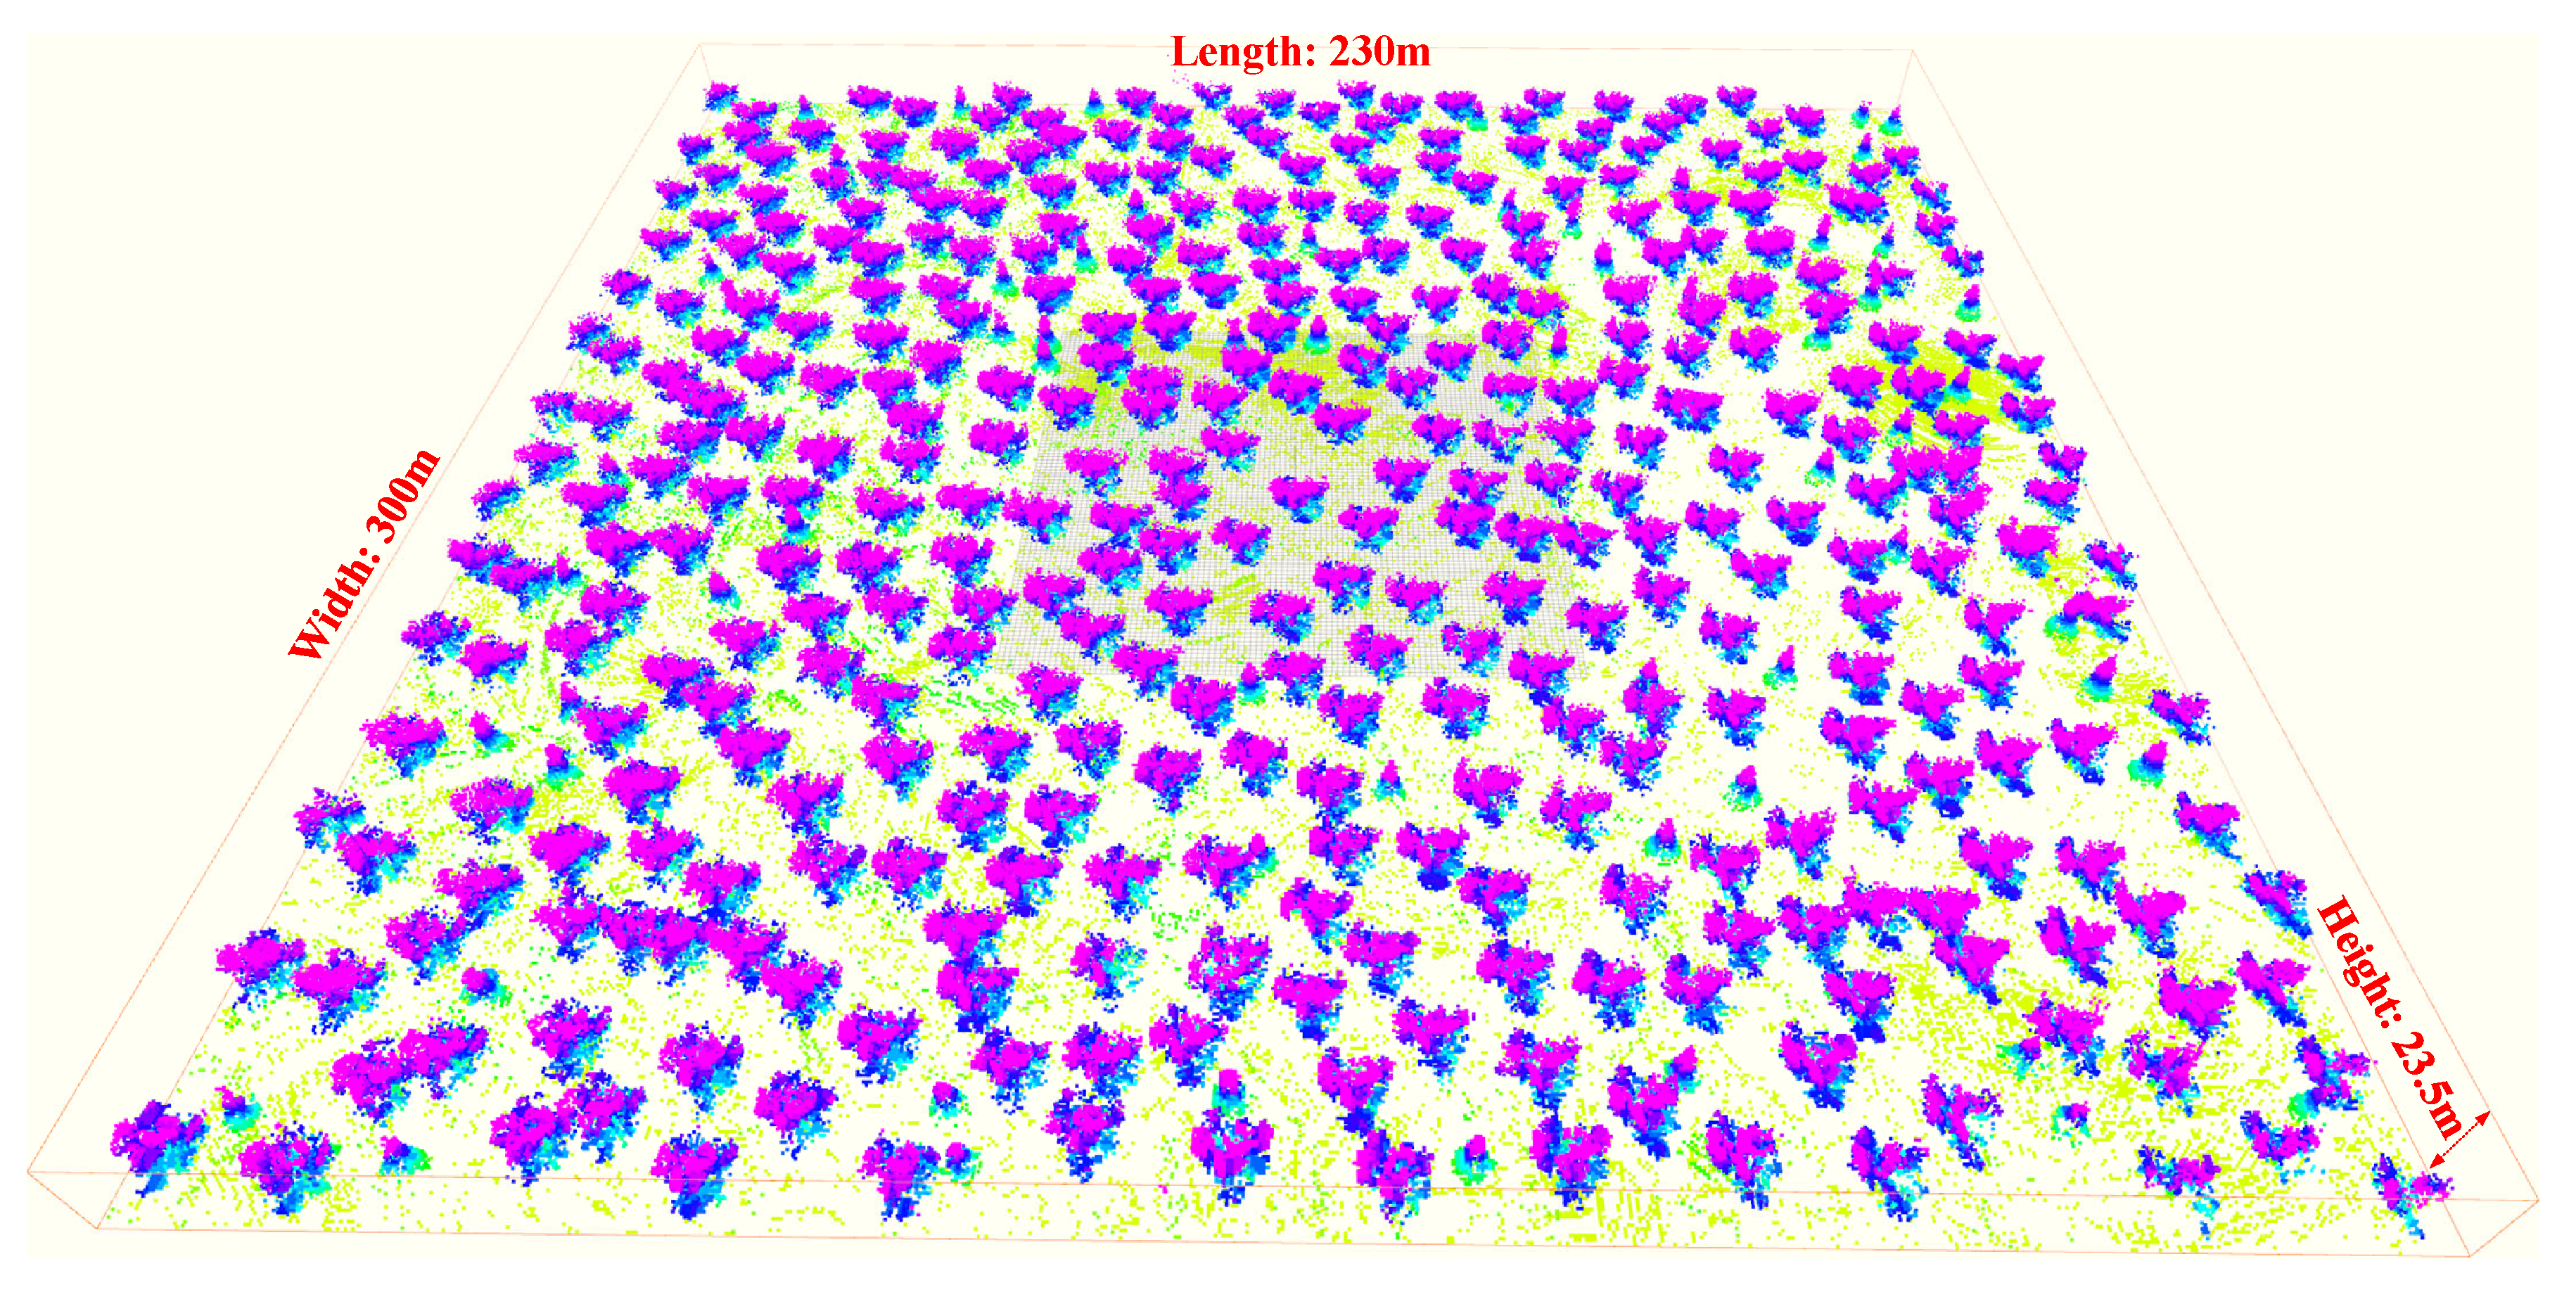
\includegraphics[width=0.745\columnwidth]{s3.pdf}}  
  \caption{\label{fig_env} The exploration scenarios. (a) The building cluster scene reconstructed in 3D from a real office building, covering an area of $125\text{ m} \times 125\text{ m}$, featuring dense buildings and greenery. (b) The small village scene with an area of $200\text{ m} \times 200\text{ m}$, featuring a cluster of buildings and scattered woods.  (c) The forest scene with an area of $300\text{ m} \times 300\text{ m}$, featuring dense trees.}
  % \vspace{-0.4cm}
\end{figure*}

This section conducted extensive simulations and hardware-in-the-loop experiments to evaluate the proposed method against two state-of-the-art (SOTA) algorithms, namely RACER \cite{zhou2023racer} and Bartolomei et al. \cite{bartolomei2023fast}. Note that both algorithms involved in the comparison are originally based on vision sensors. To ensure a fair comparison, we adapted them to be compatible with LiDAR. 
We selected two challenging, large-scale environments, each spanning hundreds of meters and featuring dense buildings and forested areas, for multi-UAV cooperative exploration experiments, as shown in Fig. \ref{fig_env}. 
Meanwhile, all simulations and hardware-in-the-loop experiments are conducted using the Gazebo simulator on a desktop with an Intel Core i9-14900KF CPU and an RTX 3090 GPU. In the hardware-in-the-loop experiments, it is important to note that all exploration algorithms are deployed on the RK3588S computing platform. Furthermore, each UAV in the exploration process is equipped with a simulated 360-degree Livox MID360 LiDAR, with a detection range set to 30 m. The UAV's maximum linear and angular velocities are set to 3.5 m/s and 1.0 rad/s, respectively. 
In exploration experiments, a test is considered successful when the UAVs achieve over $95\%$ effective coverage of the environment. The exploration is terminated once no new frontiers can be extracted or the exploration duration exceeds 1200 s.

\subsection{Benchmark and Comparisons}
\label{subsec:sim_benchmark}

\begin{table*}[thpb]
\centering
\caption{Exploration Statistics}
% \vspace{-0.2cm}
	\begin{tabular}{M{2.3cm}M{0.6cm}M{2.1cm}M{0.6cm}M{0.6cm}M{0.6cm}M{0.6cm}M{0.6cm}M{0.6cm}M{0.6cm}M{0.6cm}M{0.6cm}M{0.6cm}M{0.6cm}}
	\toprule\toprule
	\multirow{2}{*}{\begin{tabular}[c]{@{}c@{}}\textbf{Scenarios}\\\textbf{(m$^3$)}\end{tabular}}  & \multirow{2}{*}{\textbf{UAVs}} & \multirow{2}{*}{\textbf{Method}} & \multicolumn{4}{c}{\textbf{Exploration Time (s)}}         
																		& \multicolumn{4}{c}{\textbf{Flight Distance (m)}}          
																		& \multicolumn{2}{c}{\textbf{C.R. (\%)}} 
																		& \multirow{2}{*}{\begin{tabular}[c]{@{}c@{}}\textbf{S.R.}\\\textbf{ (\%)}\end{tabular}}\\
																	%  \cline{3-16}
									& &                                 & \textbf{Avg} & \textbf{Std} & \textbf{Max} & \textbf{Min}
																		& \textbf{Avg} & \textbf{Std} & \textbf{Max} & \textbf{Min}
																		& \textbf{Avg} & \textbf{Std}\\
	\midrule
	\multirow{6}{*}{\begin{tabular}[c]{@{}c@{}}\\Building\\Cluster\\$115\times117\times21.5$\end{tabular}} 
	& \multirow{3}{*}{\begin{tabular}[c]{@{}c@{}}N=3\end{tabular}} 
	& RACER\cite{zhou2023racer}        & 236.1 & 59.3 & 306.2 & 148.3 & \textbf{195.5} & 27.6 & \textbf{229.0} & \textbf{151.8} & 92.36 & 7.65 & 80.0 \\
	& & Bartolomei's \cite{bartolomei2023fast}    & 165.1 & \textbf{18.0} & 187.9 & 141.5 & 333.0 & 36.5 & 329.1 & 288.8 & \textbf{99.71} & \textbf{0.19} & \textbf{100.0} \\
	& & Proposed                         & \textbf{111.4} & 19.8 & \textbf{139.5} & \textbf{82.5} & {220.5} & \textbf{23.2} & {245.0} & {178.4} & {99.60} & {0.56} & \textbf{100.0} \\
	\\[-2.5ex]
	\cline{2-14}
	\\[-2.0ex]
	& \multirow{3}{*}{\begin{tabular}[c]{@{}c@{}}N=5\end{tabular}}          
	& RACER\cite{zhou2023racer}        & 174.5 & 66.9 & 284.52 & 114.6 & {121.2} & 32.0 & 158.8 & {118.4} & 91.61 & 10.34 & 80.0 \\
	& & Bartolomei's \cite{bartolomei2023fast}    & 102.3 & 17.0 & 118.0 & 70.3 & 216.8 & 40.5 & 263.4 & 143.2 & \textbf{99.91} & \textbf{0.13} & \textbf{100.0} \\
	& & Proposed                         & \textbf{58.3} & \textbf{7.0} & \textbf{70.7} & \textbf{49.8} & \textbf{116.3} & \textbf{8.5} & \textbf{132.0} & \textbf{109.0} & {99.58} & {0.42} & \textbf{100.0} \\
	\midrule
	\multirow{15}{*}{\begin{tabular}[c]{@{}c@{}}Small\\Village\\$220\times230\times23.5$\end{tabular}}  
	& \multirow{3}{*}{\begin{tabular}[c]{@{}c@{}}N=3\end{tabular}} 
	& RACER\cite{zhou2023racer}        & $>$1000 & - & $>$1000 & {864.1} & 1230.8 & 324.3 & 1779.4 & \textbf{867.6} & 81.22 & 10.59 & 20.0 \\
	& & Bartolomei's \cite{bartolomei2023fast}    & 959.5 & \textbf{13.3} & 976.9 & 938.3 & 1634.8 & \textbf{86.3} & 1741.0 & 1521.3 & 99.35 & \textbf{0.11} & \textbf{100.0} \\
	& & Proposed                         & \textbf{681.4} & 48.6 & \textbf{734.4} & \textbf{611.8} & \textbf{1335.2} & 89.0 & \textbf{1443.3} & {1245.2} & \textbf{99.64} & {0.36} & \textbf{100.0} \\
	\\[-2.5ex]
	\cline{2-14}
	\\[-2.0ex]
	& \multirow{3}{*}{\begin{tabular}[c]{@{}c@{}}N=5\end{tabular}}         
	& RACER\cite{zhou2023racer}        & $>$1000 & - & $>$1000 & 988.6 & 1611.2 & 377.2 & 1993.1 & 920.1 & 82.77 & 13.87 & 20.0 \\
	& & Bartolomei's \cite{bartolomei2023fast}    & 773.4 & 81.6 & 892.9 & 674.5 & 1126.0 & 89.7 & 1245.9 & 1026.5 & \textbf{99.97} & \textbf{0.03} & \textbf{100.0} \\
	& & Proposed                         & \textbf{490.2} & \textbf{50.0} & \textbf{576.2} & \textbf{429.0} & \textbf{937.3} & \textbf{89.1} & \textbf{1080.9} & \textbf{810.9} & {99.67} & {0.24} & \textbf{100.0} \\
	\\[-2.5ex]
	\cline{2-14}
	\\[-2.0ex]
	& \multirow{3}{*}{\begin{tabular}[c]{@{}c@{}}N=7\end{tabular}}        
	& RACER\cite{zhou2023racer}        & $>$1000 & - & $>$1000 & 524.2 & 883.1 & 327.9 & 1298.8 & \textbf{524.2} & 71.93 & 15.14 & 20.0 \\
	& & Bartolomei's \cite{bartolomei2023fast}    & 443.7 & \textbf{17.3} & 464.6 & 420.4 & 709.8 & 45.4 & 772.6 & 657.6 & 99.79 & \textbf{0.17} & \textbf{100.0} \\
	& & Proposed                         & \textbf{358.0} & 23.2 & \textbf{375.8} & \textbf{314.8} & \textbf{649.9} & \textbf{45.1} & \textbf{708.7} & {569.9} & \textbf{99.83} & {0.22} & \textbf{100.0} \\
	\\[-2.5ex]
	\cline{2-14}
	\\[-2.0ex]
	& \multirow{3}{*}{\begin{tabular}[c]{@{}c@{}}N=9\end{tabular}} 
	& RACER\cite{zhou2023racer}        & $>$1000 & - & $>$1000 & 999.1 & 1013.6 & 444.6 & 1476.7 & 257.6 & 80.25 & 11.45 & 20.0 \\
	& & Bartolomei's \cite{bartolomei2023fast}    & 339.7 & \textbf{15.9} & 370.5 & 327.0 & 533.9 & \textbf{18.3} & 559.1 & 510.3 & \textbf{99.99} & \textbf{0.01} & \textbf{100.0} \\
	& & Proposed                         & \textbf{257.7} & 17.9 & \textbf{286.2} & \textbf{234.7} & \textbf{443.4} & 20.7 & \textbf{484.6} & \textbf{429.5} & \textbf{99.99} & \textbf{0.01} & \textbf{100.0} \\
	% \\[-2.5ex]
	% \cline{2-14}
	% \\[-2.0ex]
	% & \multirow{3}{*}{\begin{tabular}[c]{@{}c@{}}N=10\end{tabular}}         
	% & RACER\cite{zhou2023racer}        & 114.0 & 5.80 & 120.3 & 101.9 & 176.4 & 10.95 & 192.5 & 149.3 & 880.9 & 1.44 & 882.7 \\
	% & & Bartolomei's \cite{bartolomei2023fast}    & 115.1 & 4.96 & 126.4 & 108.0 & 167.4 & 14.34 & 193.9 & 152.6 & 881.0 & 1.89 & 884.0 \\
	% & & Proposed                         & \textbf{291.9} & 6.56 & 298.4 & 280.1 & \textbf{495.7} & 16.64 & 511.4 & 464.0 & \textbf{4212.8} & 4.08 & 100.0 \\
	\midrule
	\multirow{15}{*}{\begin{tabular}[c]{@{}c@{}}Forest\\$300\times300\times15.5$\end{tabular}}  
	& \multirow{3}{*}{\begin{tabular}[c]{@{}c@{}}N=3\end{tabular}} 
	& RACER\cite{zhou2023racer}        & $>$1500 & - & $>$1500 & $>$1500 & - & - & - & - & 65.67 & 16.27 & 0.0 \\
	& & Bartolomei's \cite{bartolomei2023fast}    & 1266.9 & \textbf{72.5} & 1386.8 & 1182.0 & 2278.9 & \textbf{99.1} & 2448.6 & 2145.7 & 99.60 & \textbf{0.35} & \textbf{100.0} \\
	& & Proposed                         & \textbf{967.6} & {122.7} & \textbf{1176.7} & \textbf{833.7} & \textbf{1759.4} & 208.6 & \textbf{2002.1} & \textbf{1516.8} & \textbf{99.64} & {0.36} & \textbf{100.0} \\
	\\[-2.5ex]
	\cline{2-14}
	\\[-2.0ex]
	& \multirow{3}{*}{\begin{tabular}[c]{@{}c@{}}N=5\end{tabular}}         
	& RACER\cite{zhou2023racer}        & $>$1500 & - & $>$1500 & $>$1500 & - & - & - & - & 71.78 & 15.82 & 0.0 \\
	& & Bartolomei's \cite{bartolomei2023fast}    & 968.6 & 57.9 & 1033.7 & 869.9 & 1724.3 & 99.8 & 1838.8 & 1540.2 & \textbf{99.91} & \textbf{0.06} & \textbf{100.0} \\
	& & Proposed                         & \textbf{597.5} & \textbf{51.3} & \textbf{679.5} & \textbf{523.9} & \textbf{1035.6} & \textbf{49.2} & \textbf{1126.3} & \textbf{982.2} & {99.90} & {0.09} & \textbf{100.0} \\
	\\[-2.5ex]
	\cline{2-14}
	\\[-2.0ex]
	& \multirow{3}{*}{\begin{tabular}[c]{@{}c@{}}N=7\end{tabular}}        
	& RACER\cite{zhou2023racer}        & $>$1500 & - & $>$1500 & 1235.9 & 849.1 & 493.0 & 1664.4 & 186.6 & 67.18 & 23.07 & 20.0 \\
	& & Bartolomei's \cite{bartolomei2023fast}    & 793.9 & 48.6 & 873.3 & 732.2 & 1408.3 & \textbf{52.8} & 1482.3 & 1328.2 & \textbf{99.95} & \textbf{0.04} & \textbf{100.0} \\
	& & Proposed                         & \textbf{457.8} & \textbf{39.2} & \textbf{529.4} & \textbf{415.6} & \textbf{801.9} & 91.9 & \textbf{981.0} & \textbf{729.5} & {99.87} & {0.09} & \textbf{100.0} \\
	\\[-2.5ex]
	\cline{2-14}
	\\[-2.0ex]
	& \multirow{3}{*}{\begin{tabular}[c]{@{}c@{}}N=9\end{tabular}} 
	& RACER\cite{zhou2023racer}        & $>$1500 & - & $>$1500 & $>$1500 & - & - & - & - & - & 8.74 & 0.0 \\
	& & Bartolomei's \cite{bartolomei2023fast}    & 763.0 & 122.9 & 1005.8 & 678.9 & 1350.9 & 118.7 & 1578.4 & 1238.7 & \textbf{99.99} & \textbf{0.01} & \textbf{100.0} \\
	& & Proposed                         & \textbf{415.2} & \textbf{28.9} & \textbf{466.8} & \textbf{380.4} & \textbf{623.2} & \textbf{13.2} & \textbf{642.1} & \textbf{608.8} & \textbf{99.99} & \textbf{0.01} & \textbf{100.0} \\
	\\[-2.5ex]
	\cline{2-14}
	\\[-2.0ex]
	& \multirow{3}{*}{\begin{tabular}[c]{@{}c@{}}N=10\end{tabular}}         
	& RACER\cite{zhou2023racer}        & $>$1500 & - & $>$1500 & 599.3 & 599.9 & 233.4 & 816.5 & 151.9 & 73.28 & 21.28 & 20.0 \\
	& & Bartolomei's \cite{bartolomei2023fast}    & 777.0 & 112.9 & 915.0 & 630.1 & 1405.7 & 218.1 & 1703.4 & 1130.2 & \textbf{99.99} & \textbf{0.01} & \textbf{100.0} \\
	& & Proposed                         & \textbf{363.9} & \textbf{19.2} & \textbf{395.1} & \textbf{338.7} & \textbf{590.0} & \textbf{45.5} & \textbf{660.2} & \textbf{530.5} & \textbf{99.99} & \textbf{0.01} & \textbf{100.0} \\
	\toprule\toprule
	% \vspace{-0.4cm}
\end{tabular}
\label{tab:sim_result}
\end{table*}

In the simulations, we evaluate the proposed MAPPER algorithm against the abovementioned algorithms in two challenging scenarios, as shown in Fig. \ref{fig_env}. Specifically, in the real-world reconstruction scenario, we conducted three cooperative exploration experiments with varying numbers of UAVs, repeating each experiment 5 times. In the 3D digital scenario, we performed six cooperative exploration experiments with varying numbers of UAVs, repeating each experiment 5 times. It is important to note that communication between UAVs is assumed to be perfect throughout the experiments. The results for each algorithm in both scenarios are summarized in Table \ref{tab:sim_result}, which presents three key metrics: exploration time, average UAV flight distance, and the effective exploration coverage rate of the environment.

By observing Table \ref{tab:sim_result}, we can find that our proposed MAPPER significantly outperforms the other two algorithms regarding exploration time. Specifically, compared to the algorithm with the second shortest exploration time,  the proposed MAPPER reduces the exploration time by at least 13\% and up to 35\%.
Focusing further on exploration time in both scenarios, in the real-world reconstruction scenario with 5 UAVs, the proposed MAPPER algorithm completes the exploration in an average of just 85 seconds. In the 3D digital scenario, MAPPER requires only approximately 500 seconds with 10 UAVs to complete the exploration. In contrast, the other two planners took longer to complete the exploration. It is because MAPPER fully utilizes the wide detection range of LiDAR, enabling the UAV fleet to finish tasks more quickly. Moreover, MAPPER's exploration time decreases as the number of UAVs increases, demonstrating the potential of multi-UAV cooperative exploration in large-scale, challenging scenarios.
Next, we analyze the exploration coverage rate of the three algorithms. Table \ref{tab:sim_result} shows that the proposed MAPPER and the FAME algorithm completed the exploration tasks in all cases. In contrast, in most cases, the RACER algorithm failed to complete the exploration task in the larger 3D scenario. It may be because the computational load dramatically increased as the exploration area increased, causing the RACER planner to fail to calculate a reasonable exploration plan. Regarding flight distance, as shown in Table \ref{tab:sim_result}, the proposed MAPPER required the shortest flight distance in most cases. At the same time, the other two algorithms had comparable flight distances when they completed the exploration tasks.

\subsection{Effect of Communication Conditions}
\label{subsec:communications}

% \begin{figure*}[thpb]
% 	\centering
%   \subfigtopskip=0pt
% 	\subfigbottomskip=2pt
% 	\subfigcapskip=-3pt 
%   \subfigure[]{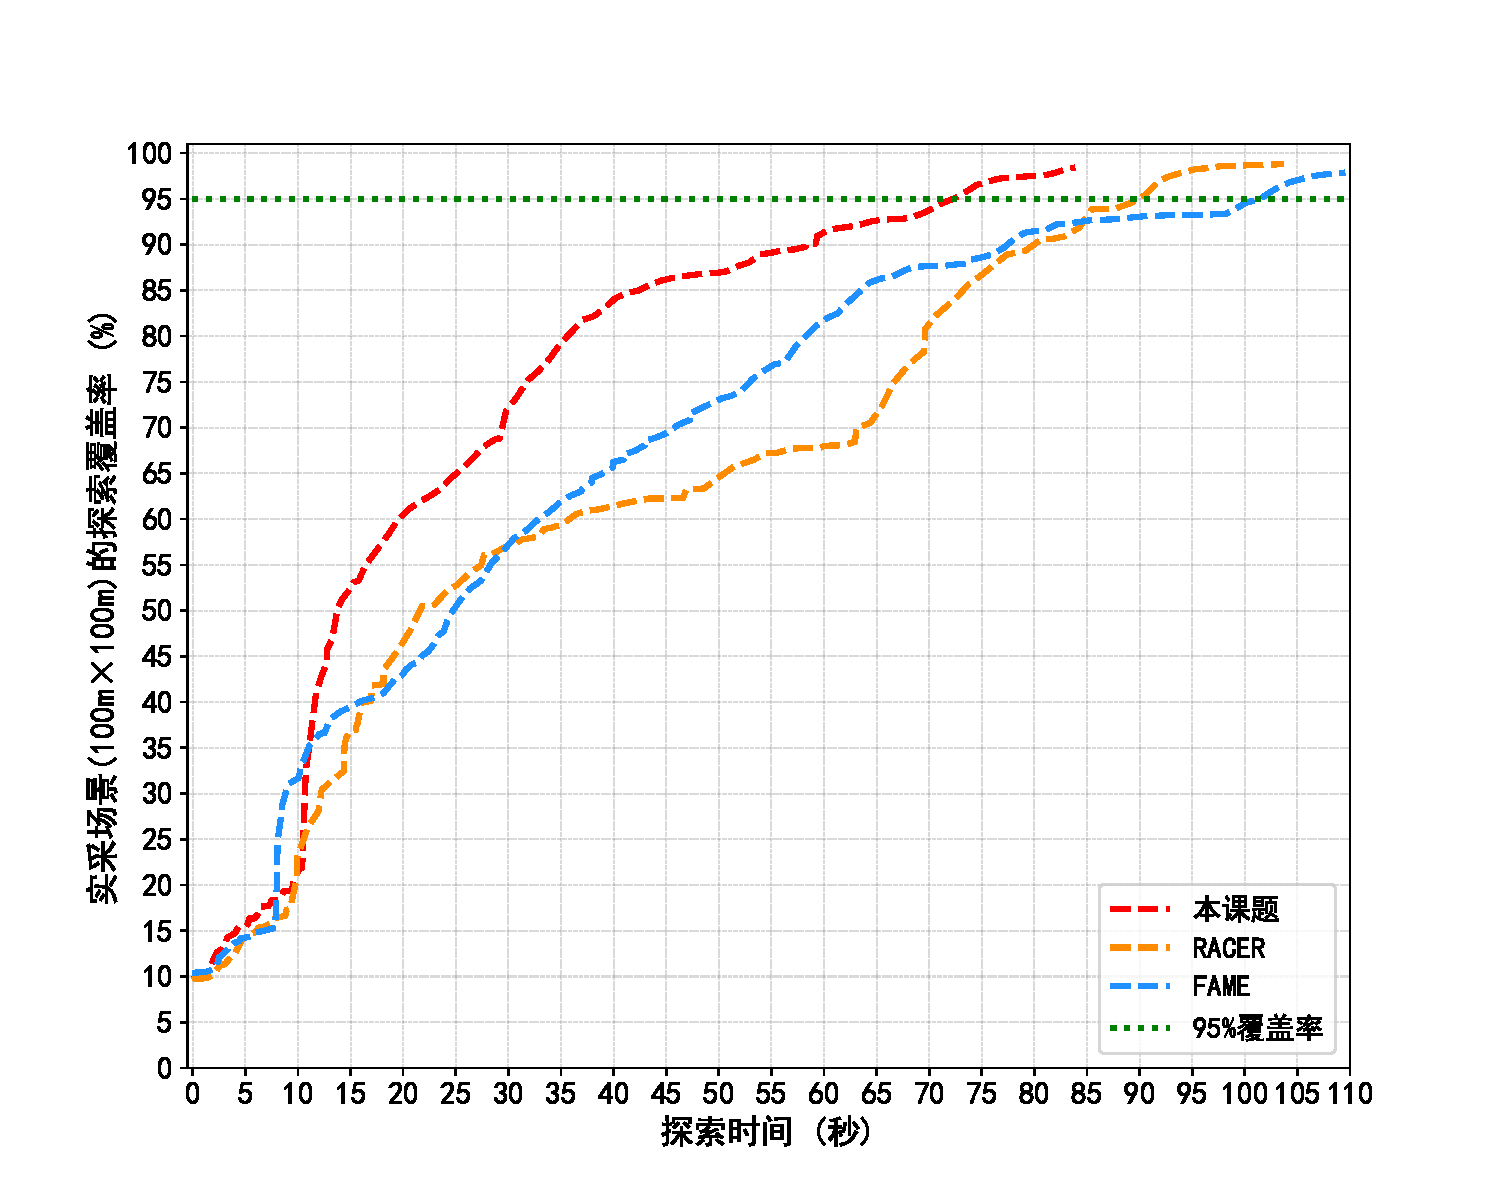
\includegraphics[width=0.65\columnwidth]{fig_explore_pro1.pdf}}
%   \subfigure[]{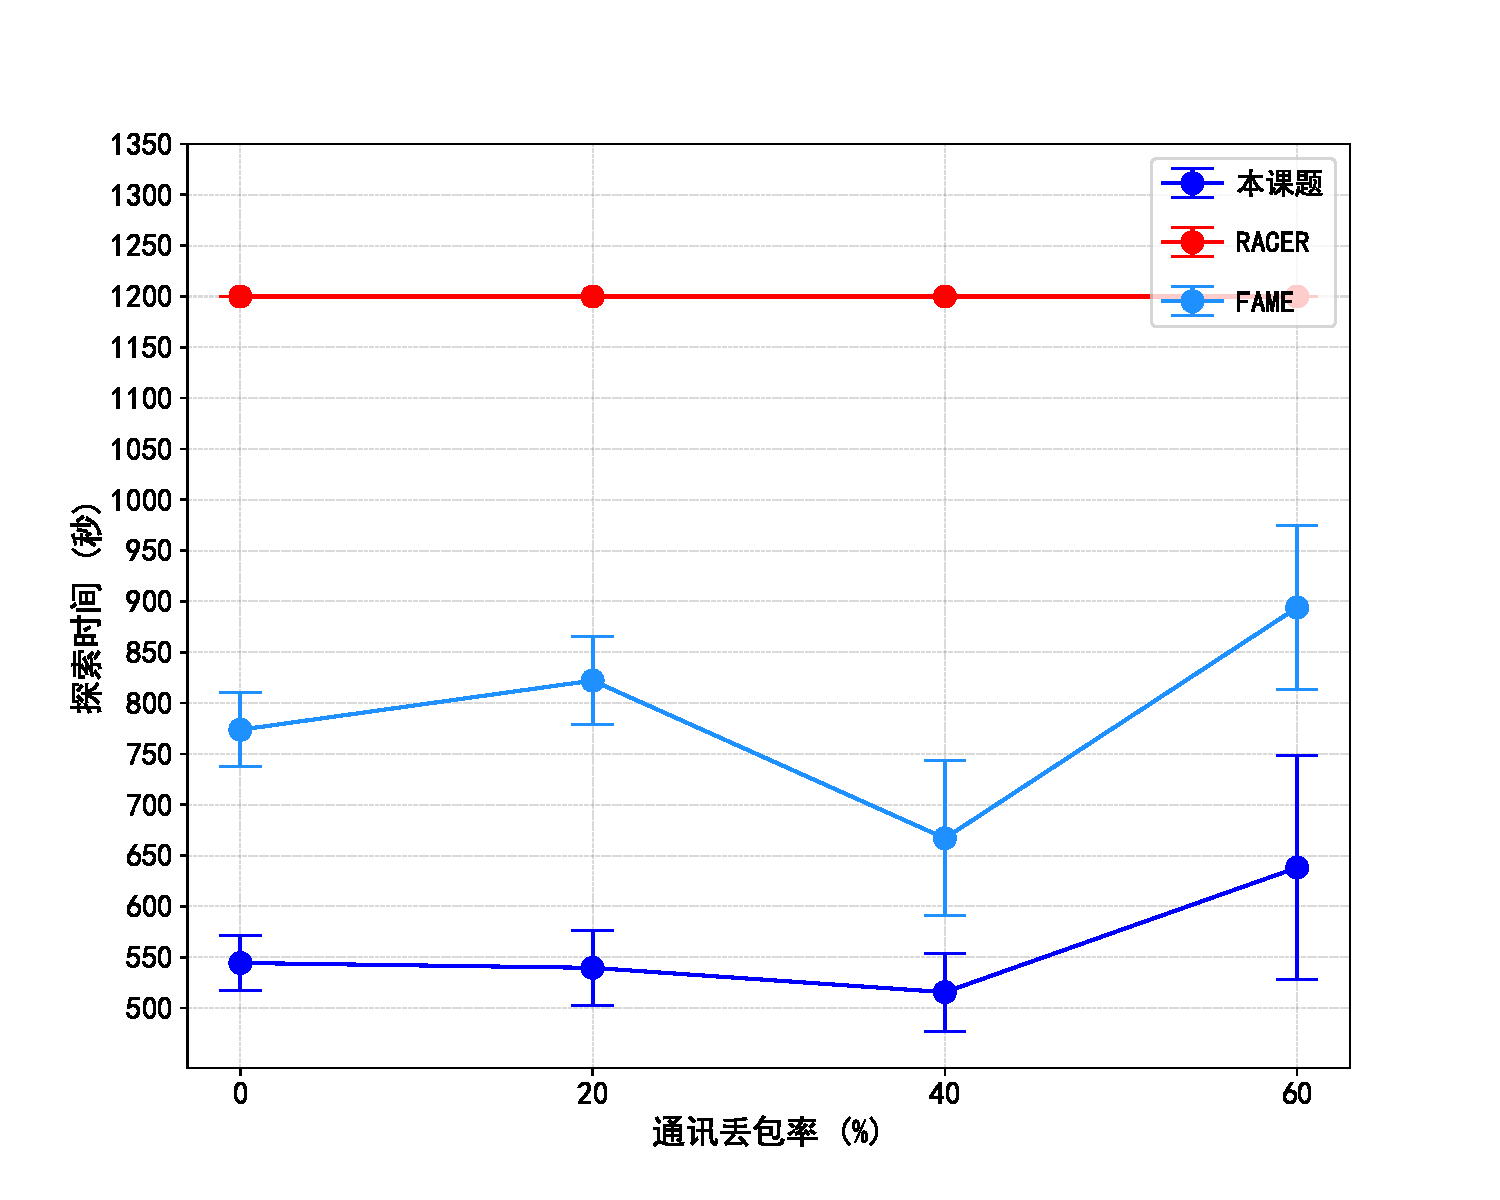
\includegraphics[width=0.65\columnwidth]{fig_loss.pdf}}
%   \subfigure[]{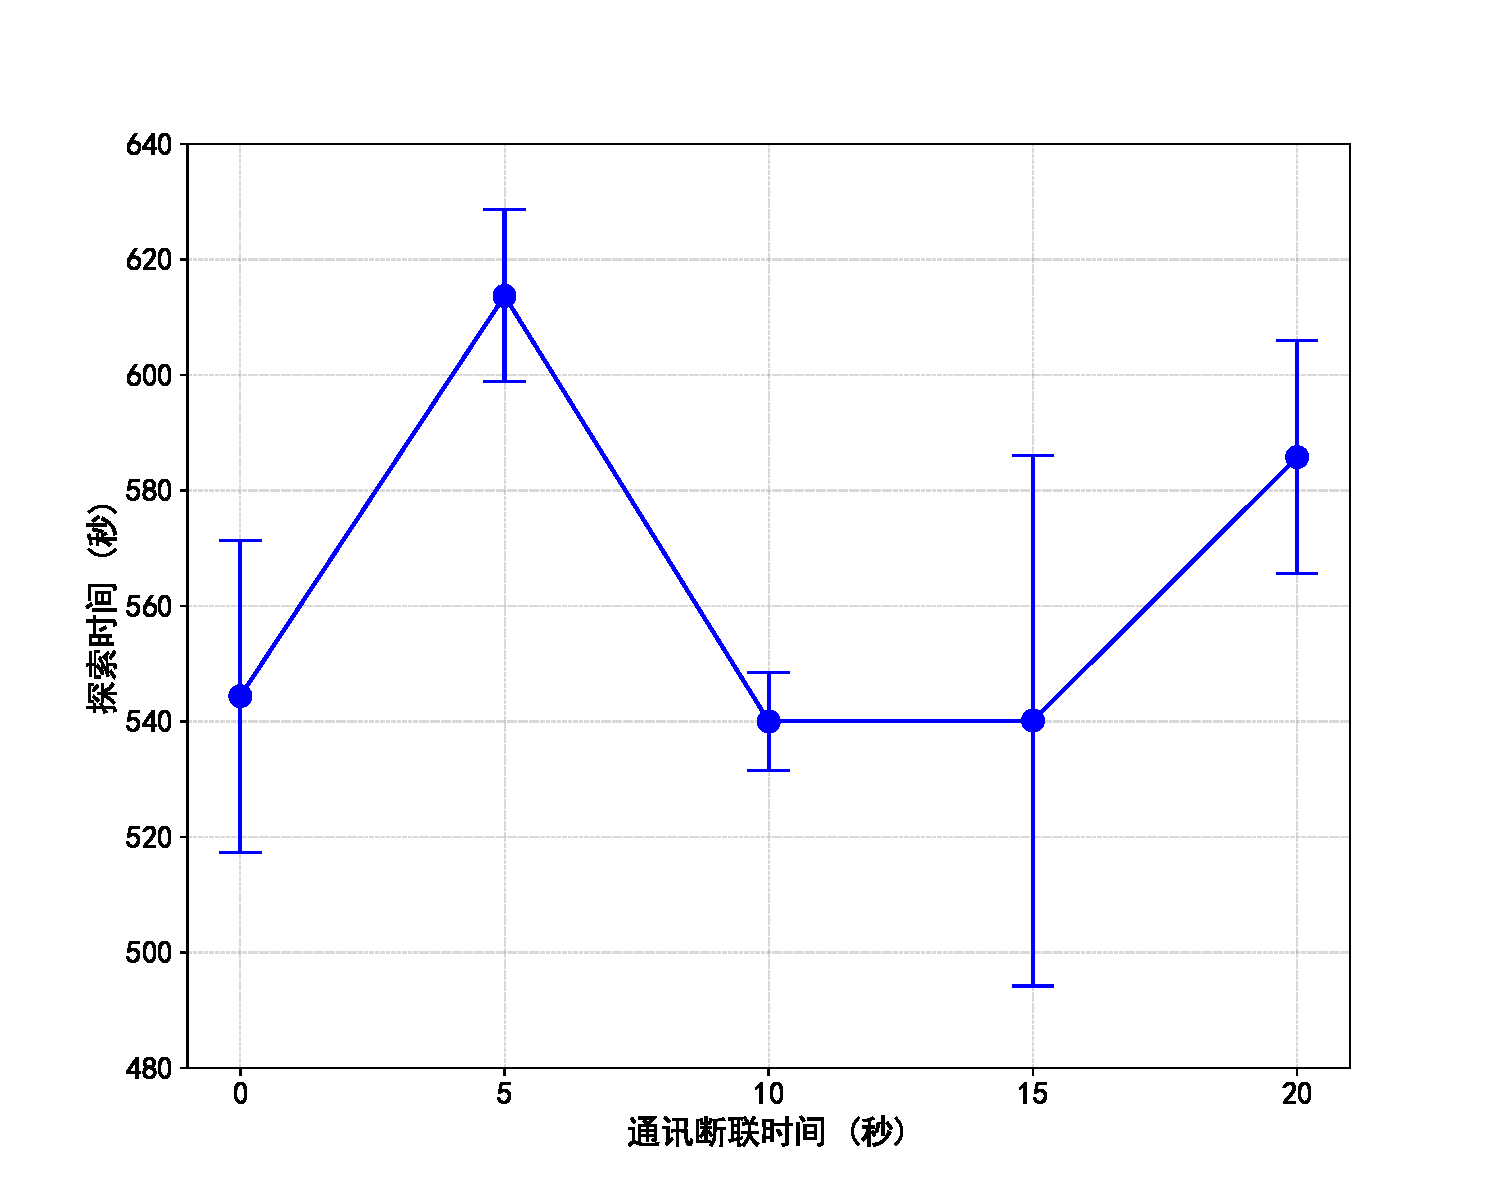
\includegraphics[width=0.64\columnwidth]{fig_disconnect.pdf}}
%   \caption{\label{fig_communication} (a) The exploration time under different packet loss rates in communication. (b) The exploration time statistics under different communication disconnection cases.}
%   % \vspace{-0.4cm}
% \end{figure*}

\begin{figure}[thpb]
	\centering
  \subfigtopskip=0pt
	\subfigbottomskip=2pt
	\subfigcapskip=-3pt 
  \subfigure[]{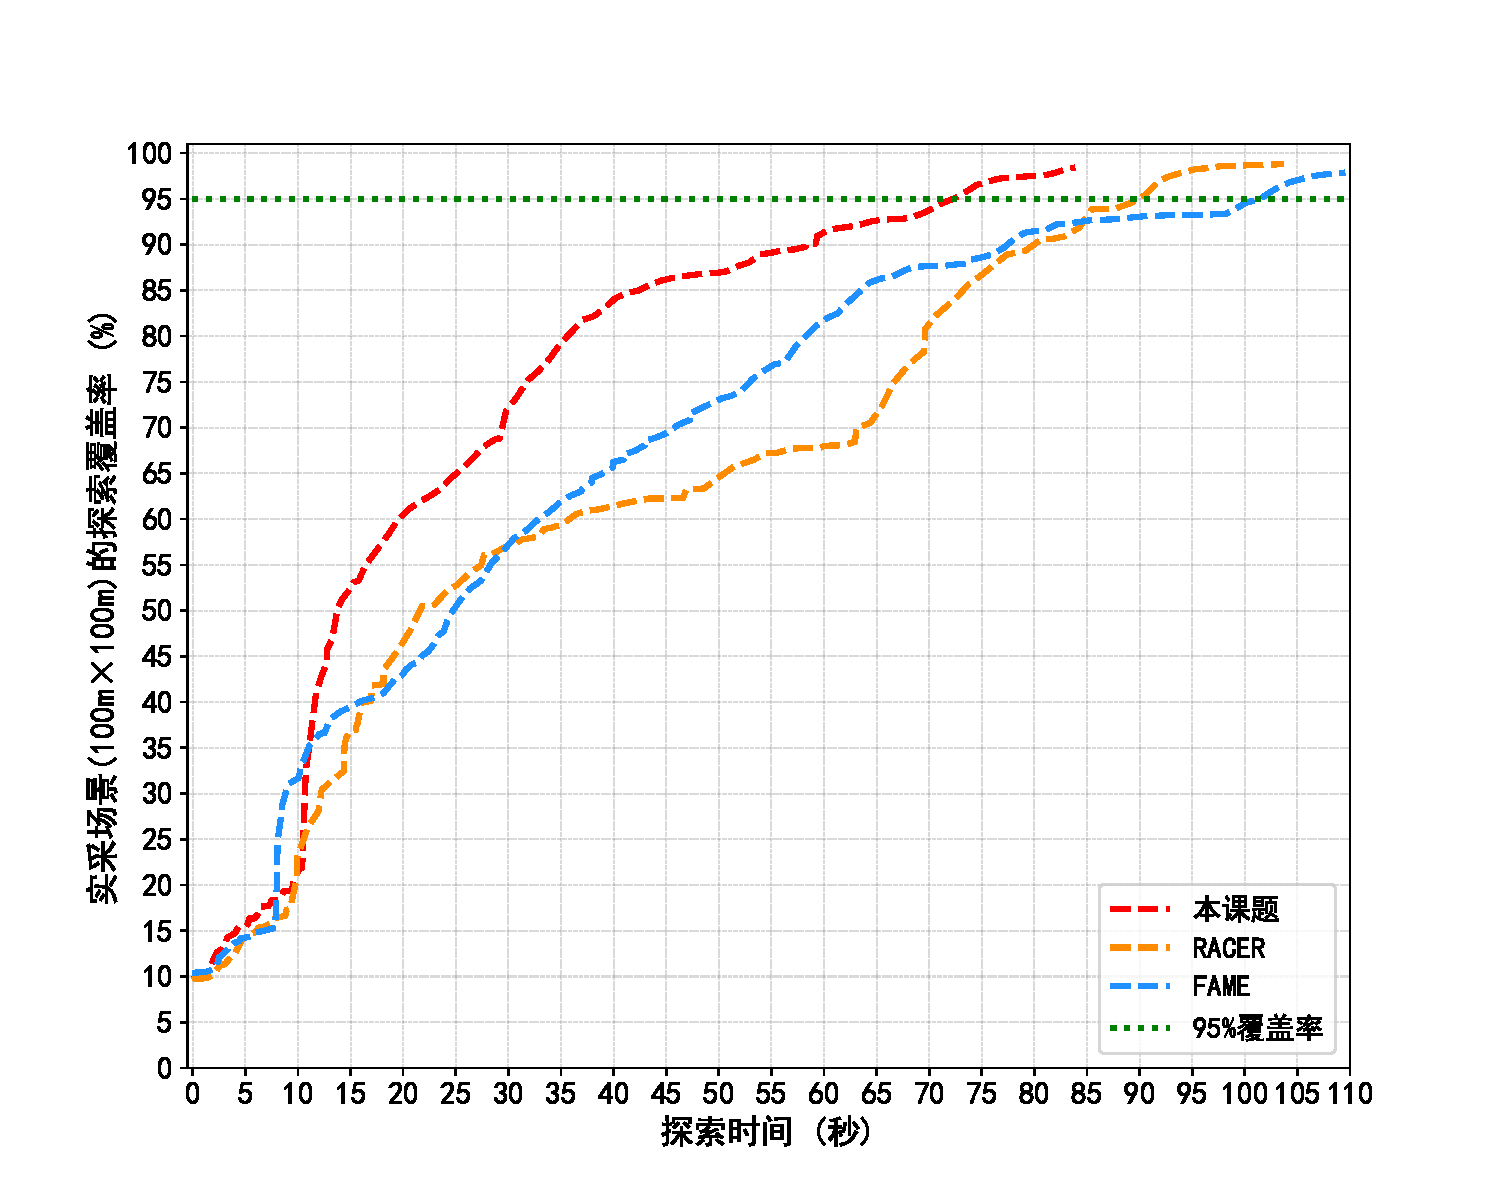
\includegraphics[width=0.32\columnwidth]{fig_explore_pro1.pdf}}
  \subfigure[]{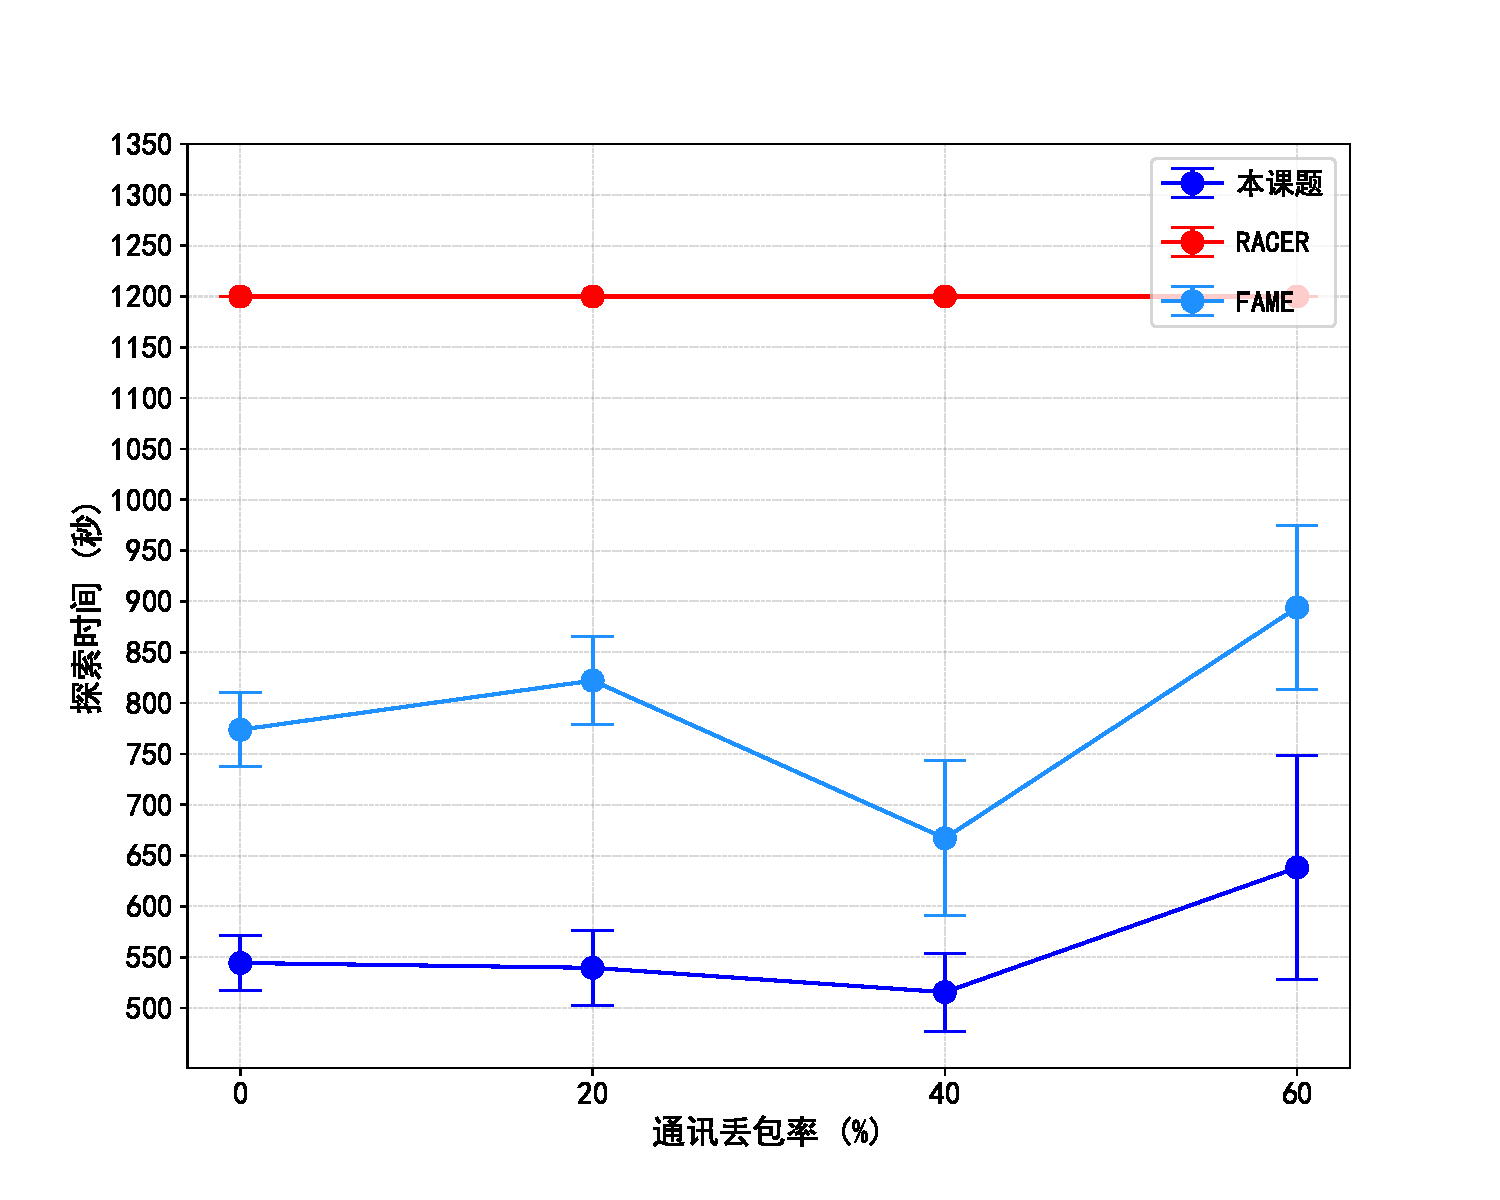
\includegraphics[width=0.32\columnwidth]{fig_loss.pdf}}
  \subfigure[]{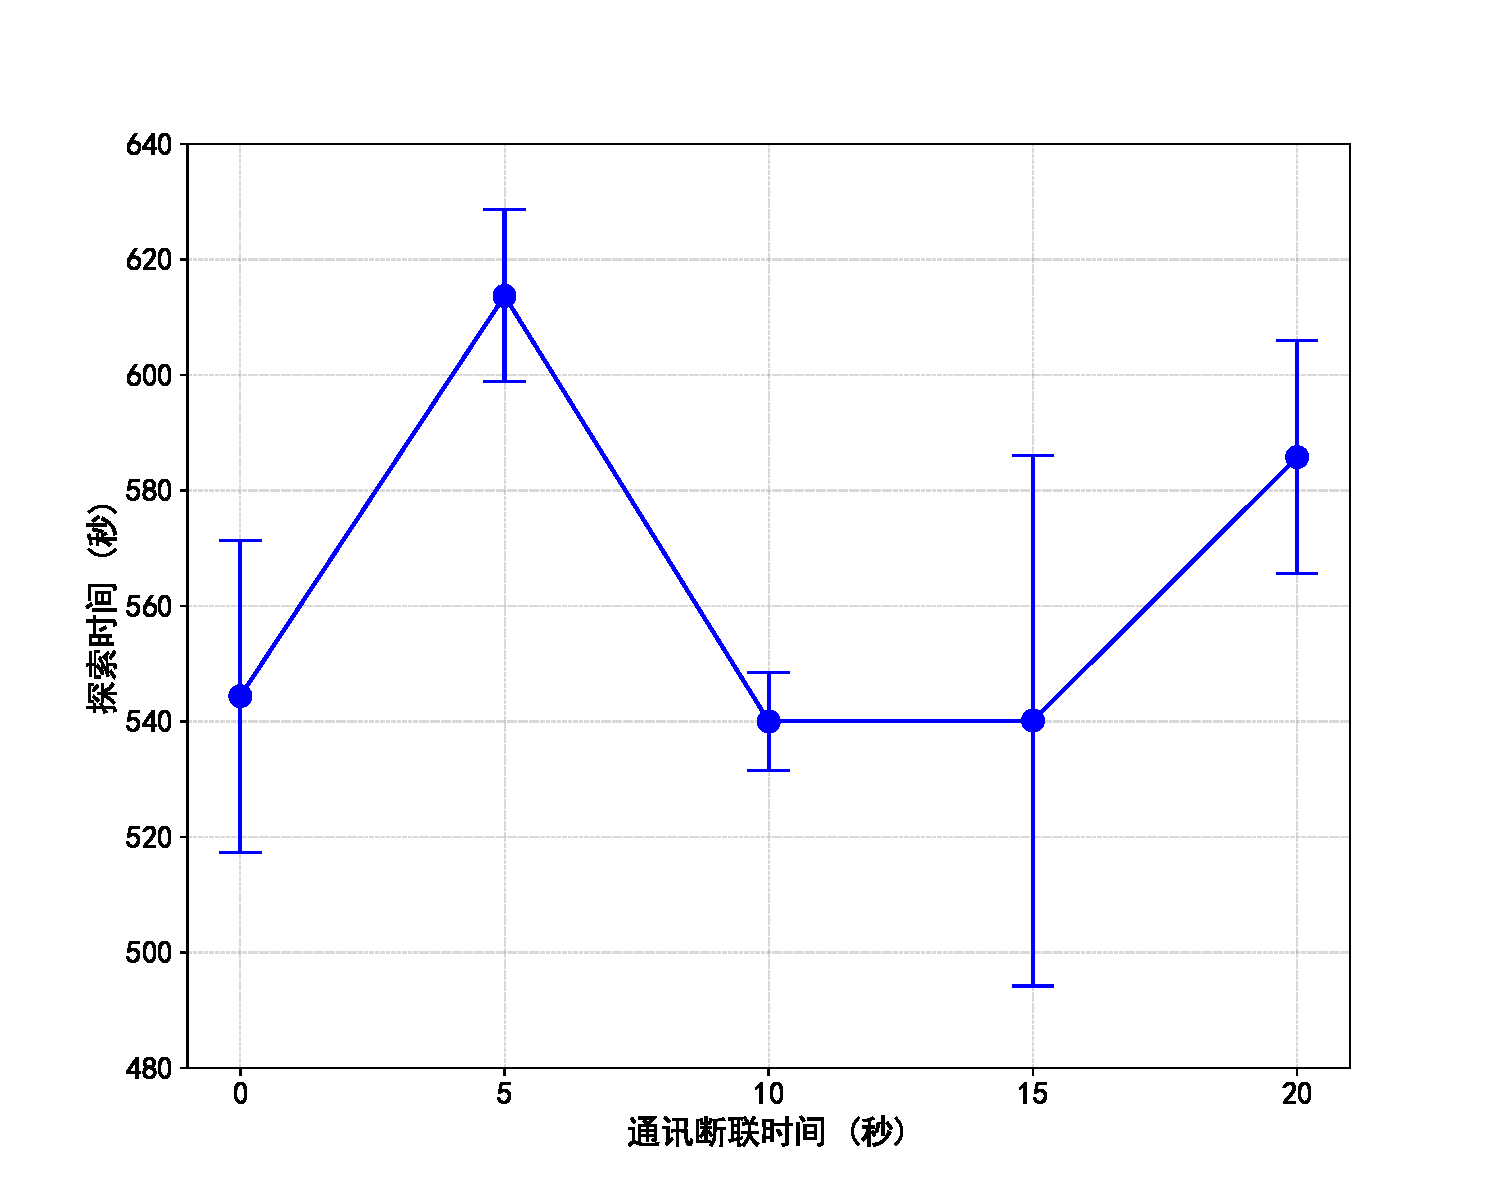
\includegraphics[width=0.32\columnwidth]{fig_disconnect.pdf}}
  \caption{\label{fig_communication} (a) The exploration time under different packet loss rates in communication. (b) The exploration time statistics under different communication disconnection cases.}
  % \vspace{-0.4cm}
\end{figure}

In this part, we evaluate the robustness of the proposed MAPPER algorithm under different communication conditions in a digital building scenario. First, we set the maximum communication range between drones to 60 meters, and then conducted five sets of exploratory experiments with different numbers of drones. Each experiment was repeated twice under the same conditions. The experimental results are shown in Fig. 6 and Fig. 7, where Fig. 6 presents the exploration time statistics of the three algorithms, and Fig. 7 shows the mapping results of the three algorithms when using 10 drones. From Fig. 6, it can be observed that despite the communication range limitations, our MAPPER algorithm consistently outperforms the others in all cases, demonstrating its strong robustness under communication constraints. Additionally, Fig. 6 shows that the FAME algorithm also successfully completed all exploration tasks, while the RACER algorithm only managed to complete the exploration task when the number of drones was limited to three, due to its high computational load.

\begin{figure}[thpb]
	\centering
  \subfigtopskip=0pt
	\subfigbottomskip=2pt
	\subfigcapskip=-3pt 
  \subfigure[]{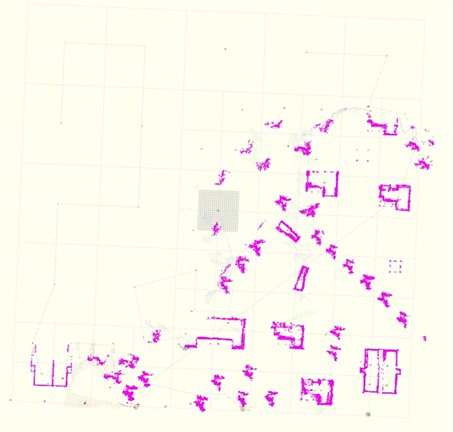
\includegraphics[width=0.32\columnwidth]{map_result_digi_racer.png}}   
  \subfigure[]{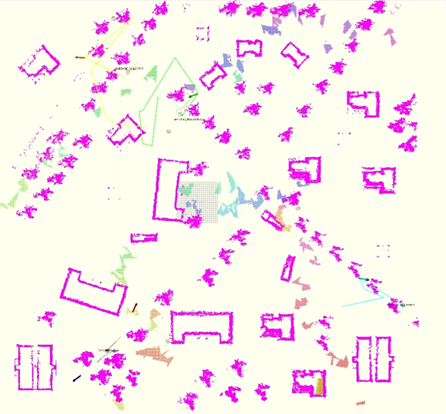
\includegraphics[width=0.32\columnwidth]{map_result_digi_fame.png}}  
  \subfigure[]{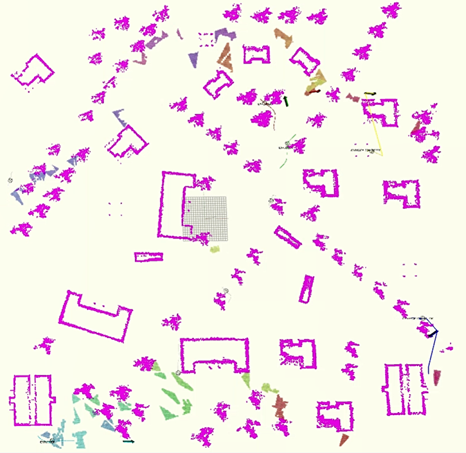
\includegraphics[width=0.32\columnwidth]{map_result_digi_mapper.png}}  
  \caption{\label{fig_map_result_digi} (a) The exploration result of RACER in 10 UAVs. (b) The exploration result of FAME in 10 UAVs. (c) The exploration result of MAPPER in 10 UAVs.}
  % \vspace{-0.6cm}
\end{figure}

To further account for the instability of the communication environment, we conducted tests with varying packet loss rates and different communication disconnection durations, based on the maximum communication distance of 60 meters. Specifically, in the experiments with different packet loss rates, the rates were set to 20\%, 40\%, and 60\%, respectively. In the disconnection experiments, we randomly disconnected drone No. 1 during the exploration process, with disconnection durations of 5 seconds, 10 seconds, 15 seconds, and 20 seconds. The experiments were conducted using 10 drones, and each communication condition was tested five times. The initial startup conditions for each algorithm were kept the same. Finally, the exploration time of the drones for the three algorithms was recorded, as shown in Fig. 8. 
Observing Fig. 8, it is clear that the MAPPER algorithm performed the best under different packet loss rates and communication disconnection durations, indicating that MAPPER can maintain higher exploration efficiency compared to the other two algorithms in unstable communication conditions. In Fig. 8(a), it can be seen that a packet loss rate of 60\% has the greatest impact on exploration efficiency, and the variance in exploration time increases as the packet loss rate rises. In Fig. 8(b), it is evident that varying communication disconnection durations have a less noticeable impact on the algorithms. This may be due to the large number of drones, which allows the remaining drones to collaborate effectively even when one experiences a communication disconnection, thus having a minimal effect on the overall exploration time. The results from Fig. 8(a) also demonstrate that the proposed MAPPER algorithm can effectively handle unexpected communication failures in drones.


\subsection{Hardware-in-the-loop Experiments}
\label{subsec:hardware simulations}

\begin{figure}[thpb]
	\centering
  \subfigtopskip=0pt
	\subfigbottomskip=2pt
	\subfigcapskip=-3pt 
  \subfigure[]{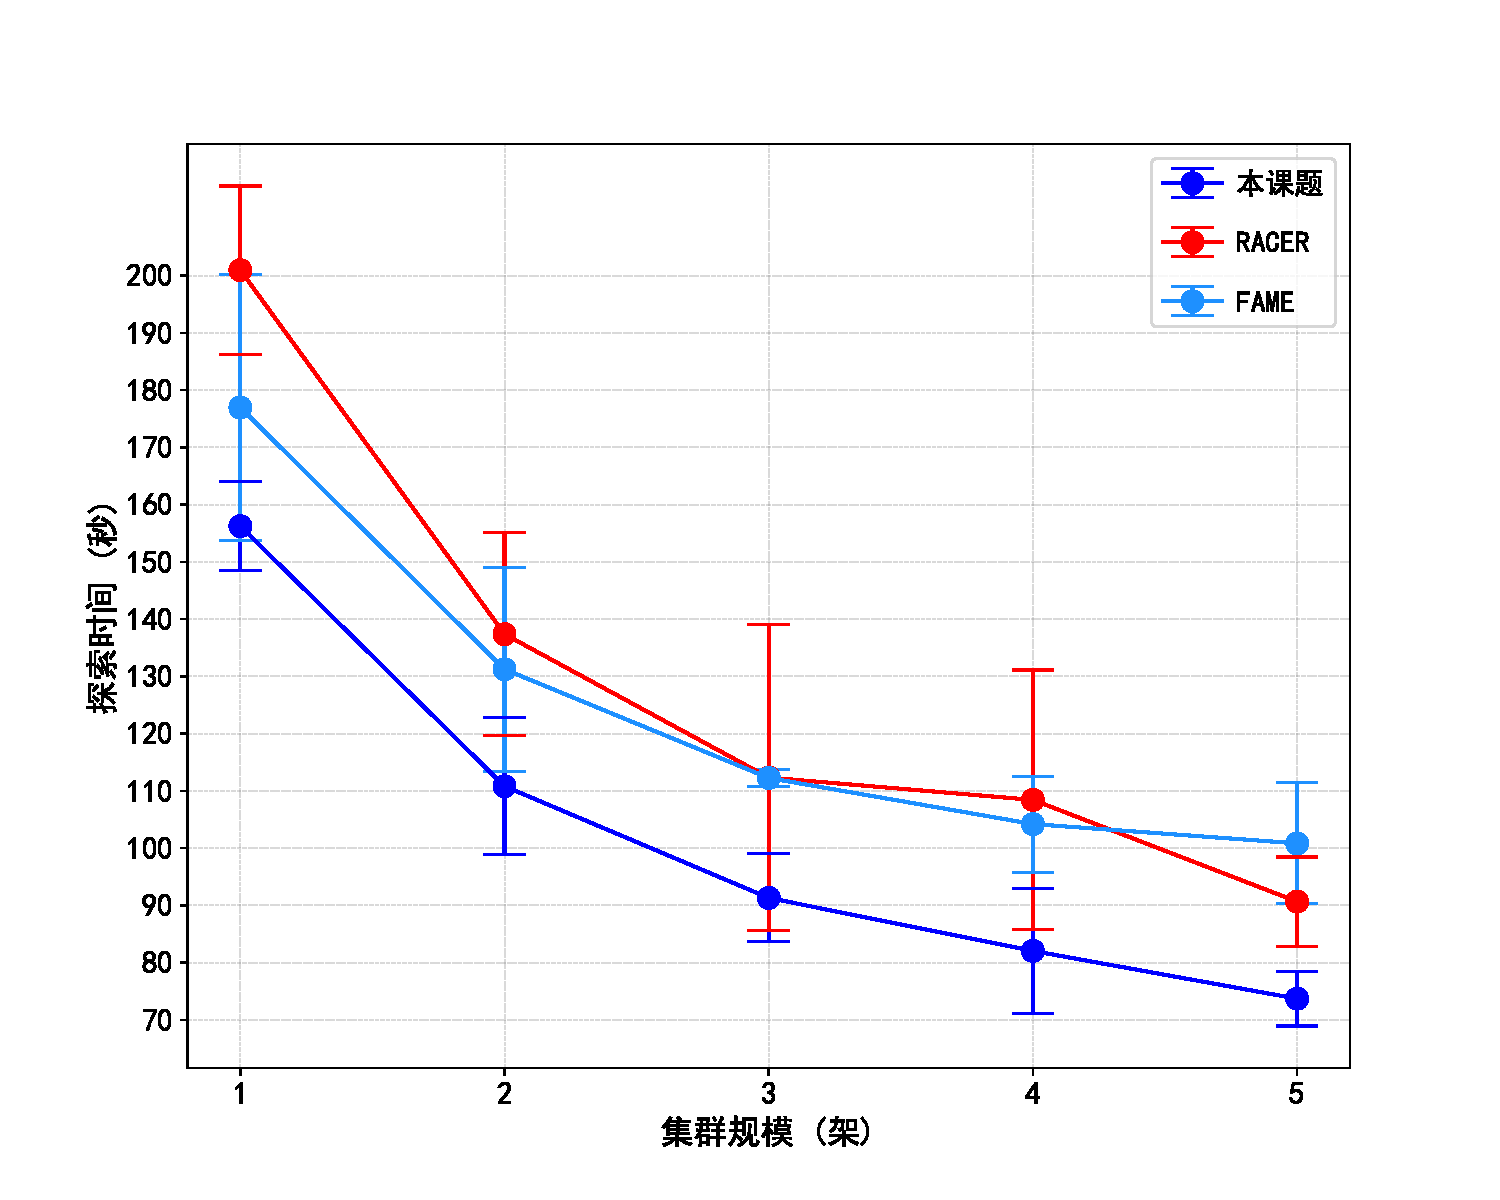
\includegraphics[width=0.32\columnwidth]{fig_real_explore_time.pdf}}
  \subfigure[]{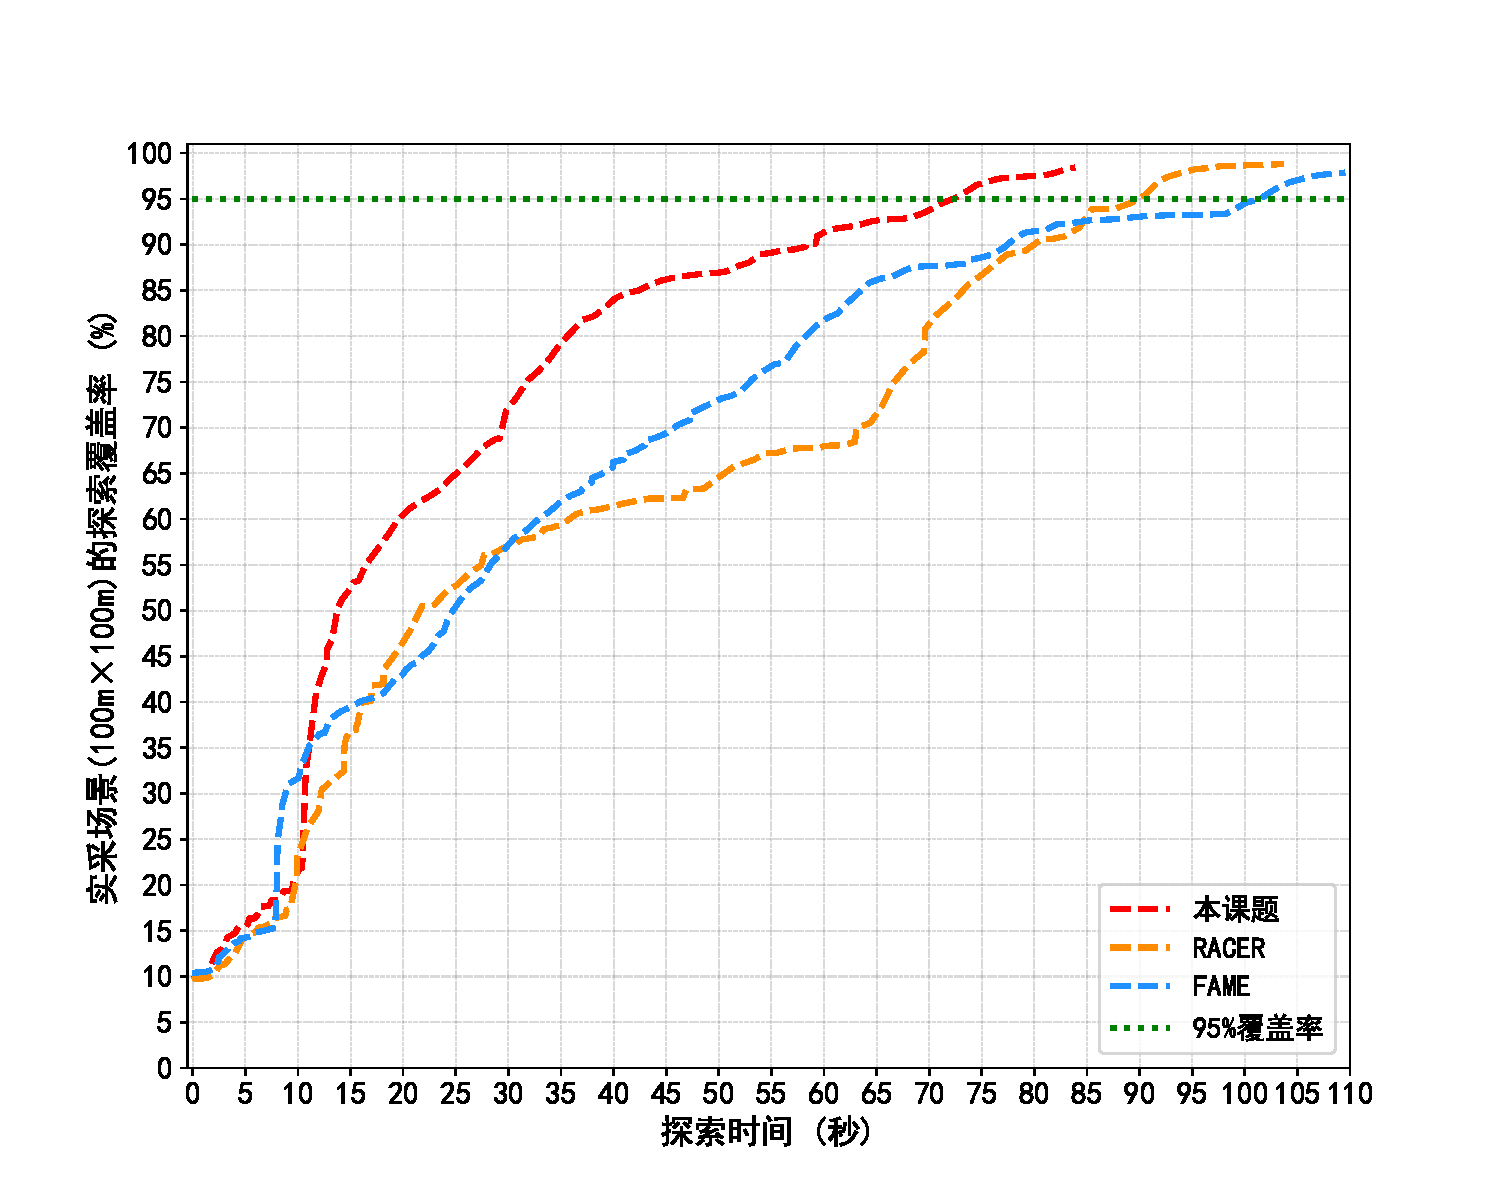
\includegraphics[width=0.32\columnwidth]{fig_explore_hard.pdf}}
  \subfigure[]{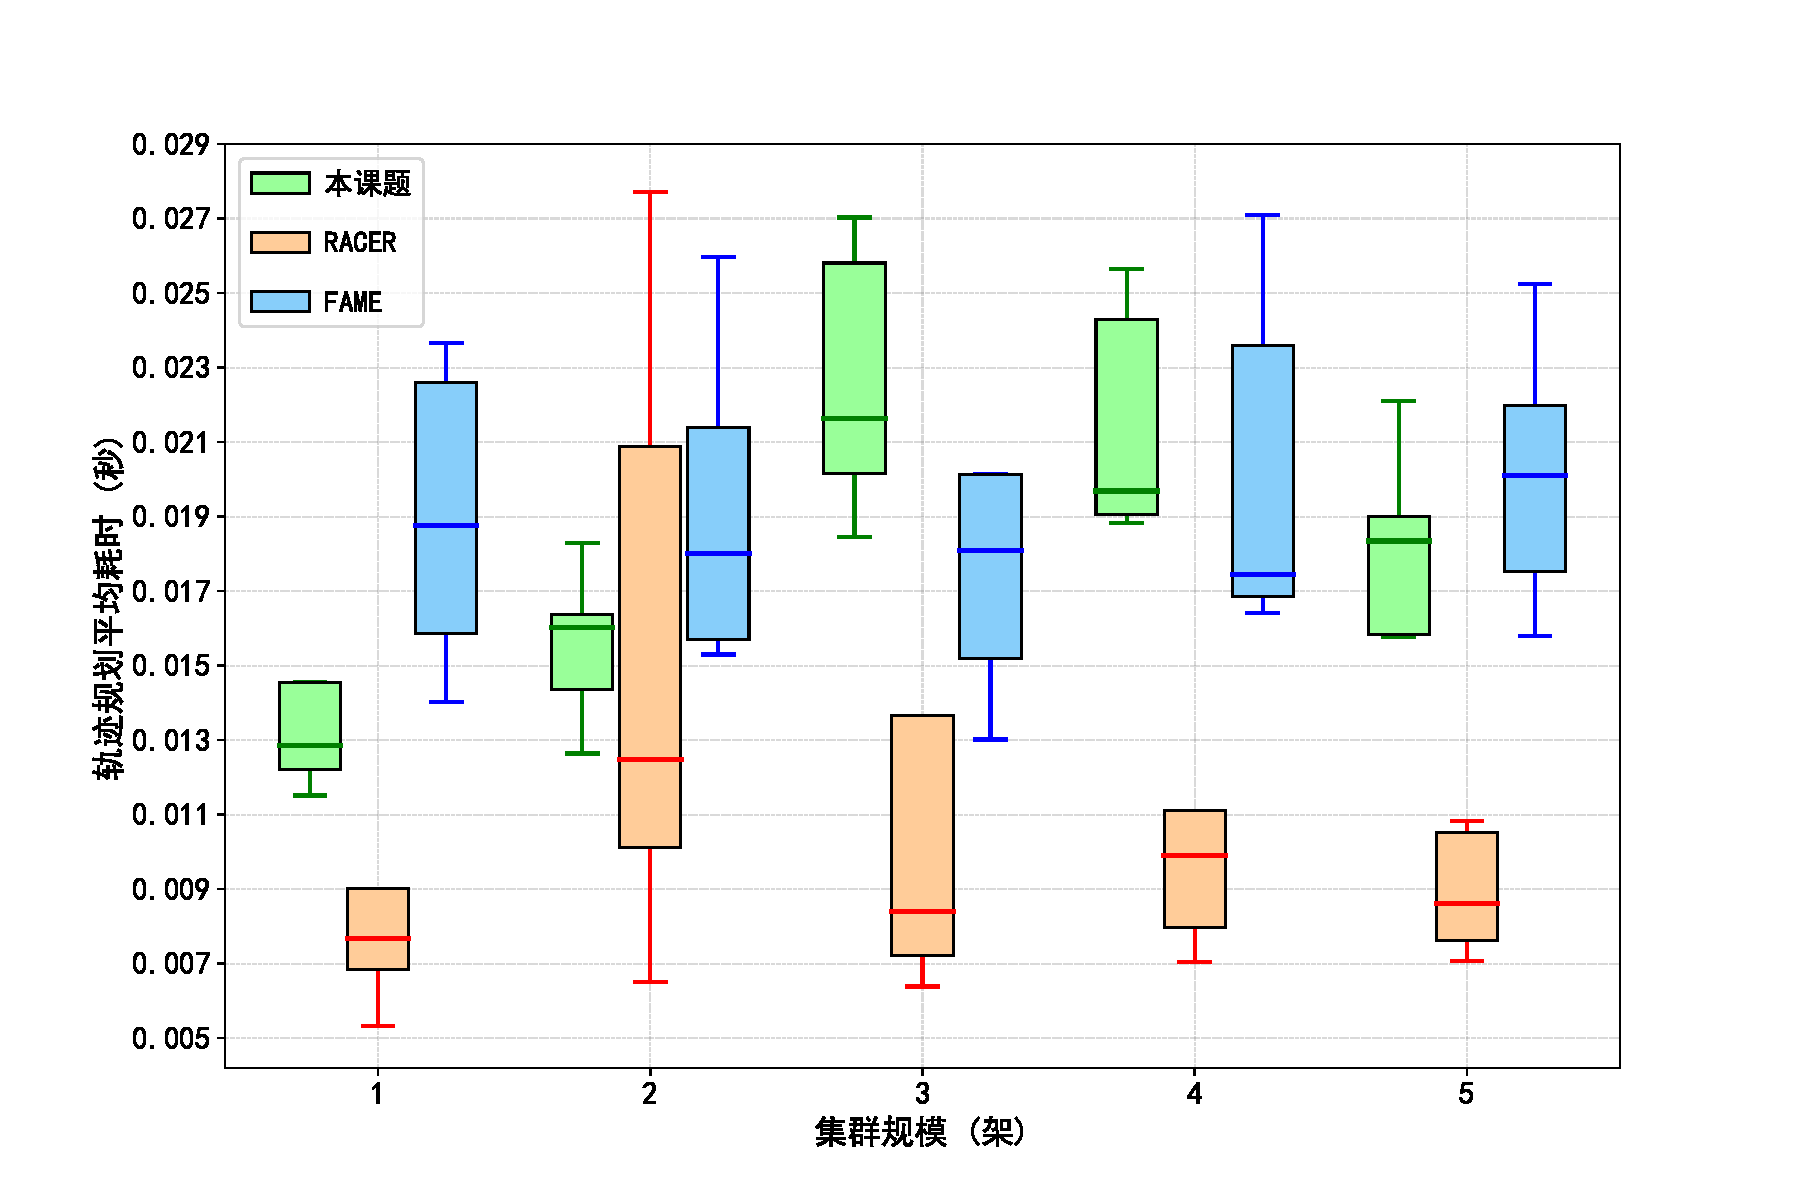
\includegraphics[width=0.32\columnwidth]{fig_compute_time.pdf}}
  \caption{\label{fig_hard_result} (a) The exploration time under different packet loss rates in communication. (b) The exploration time statistics under different communication disconnection cases.}
  % \vspace{-0.6cm}
\end{figure}

\begin{figure}[thpb]
	\centering
  \subfigtopskip=0pt
	\subfigbottomskip=2pt
	\subfigcapskip=-3pt 
  \subfigure[]{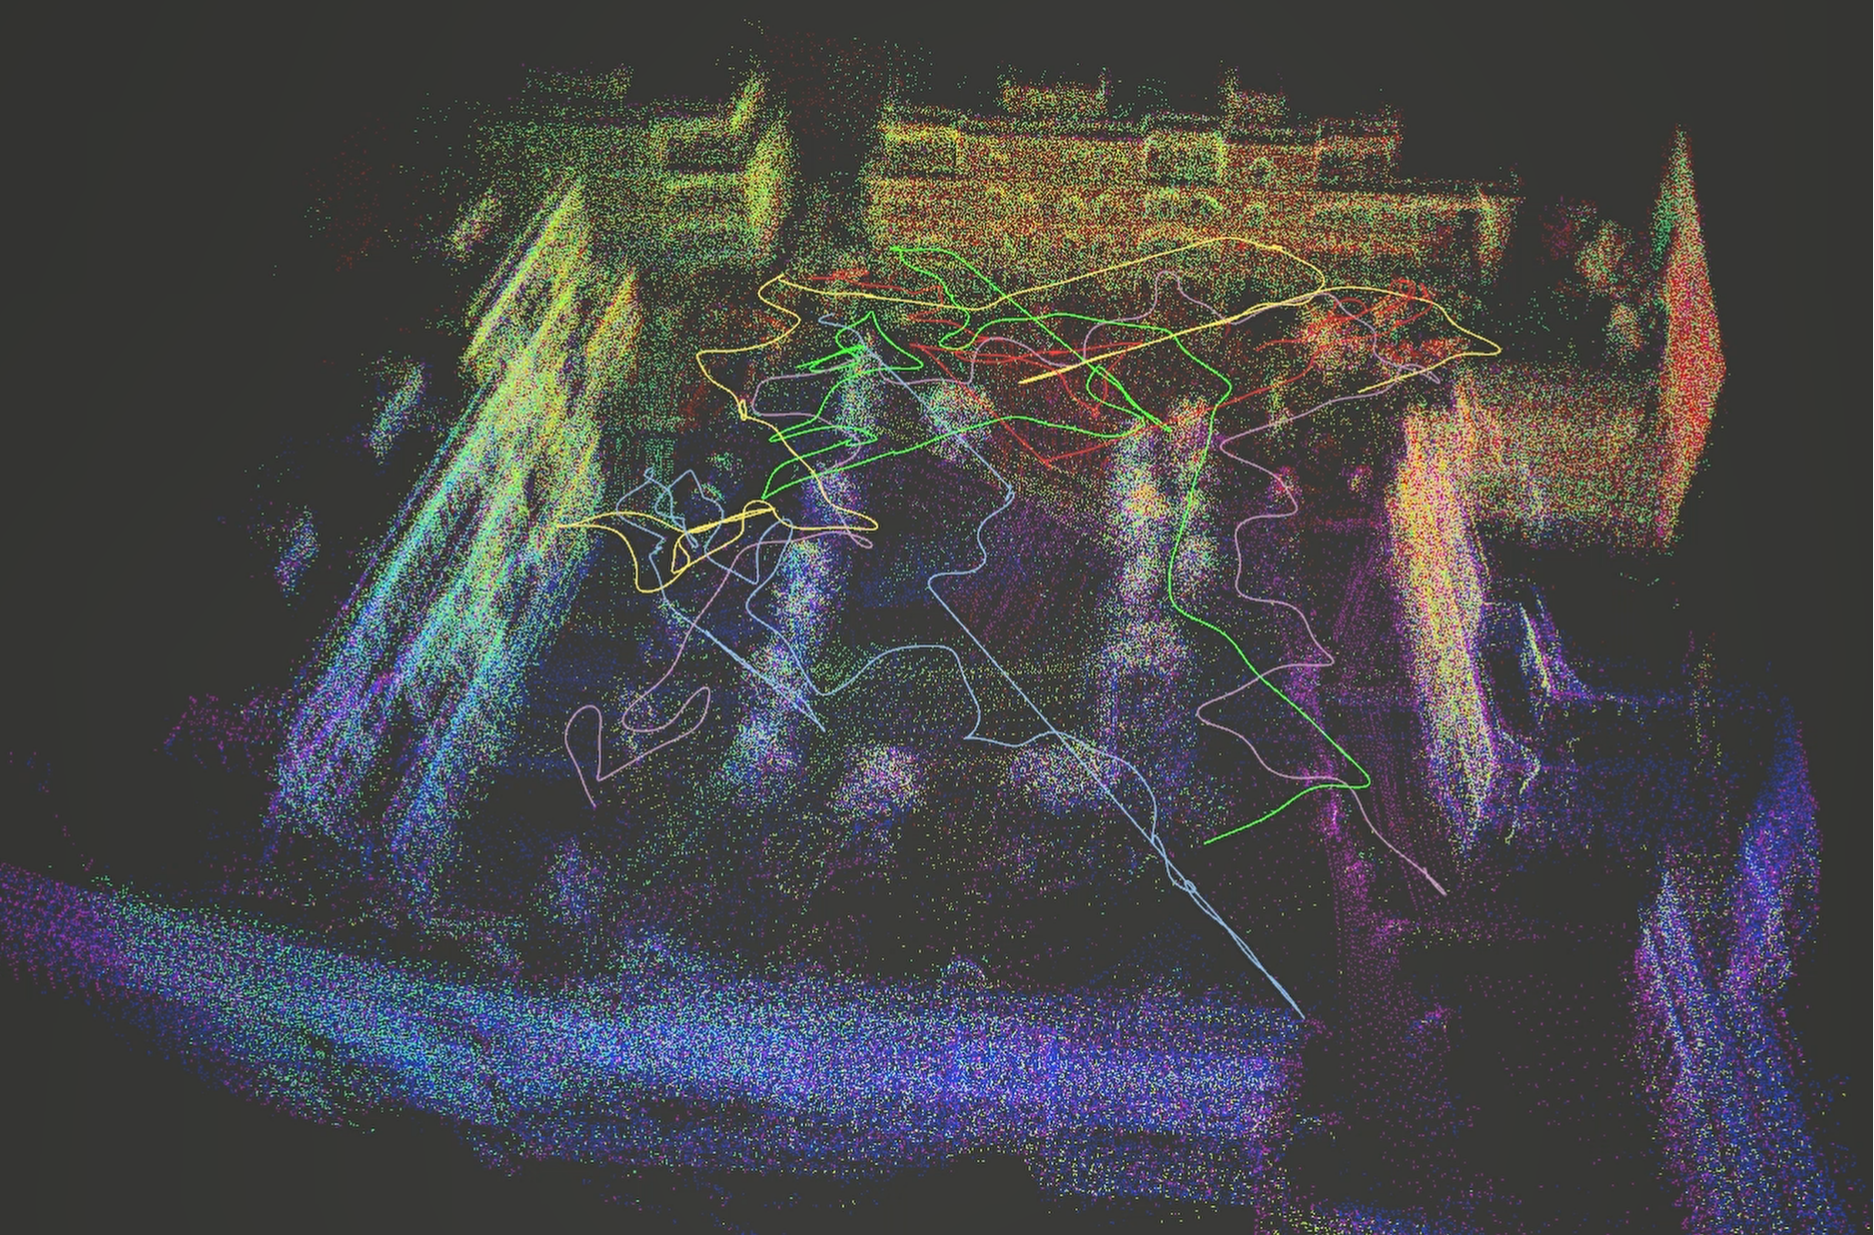
\includegraphics[width=0.32\columnwidth]{map_result_racer.png}}   
  \subfigure[]{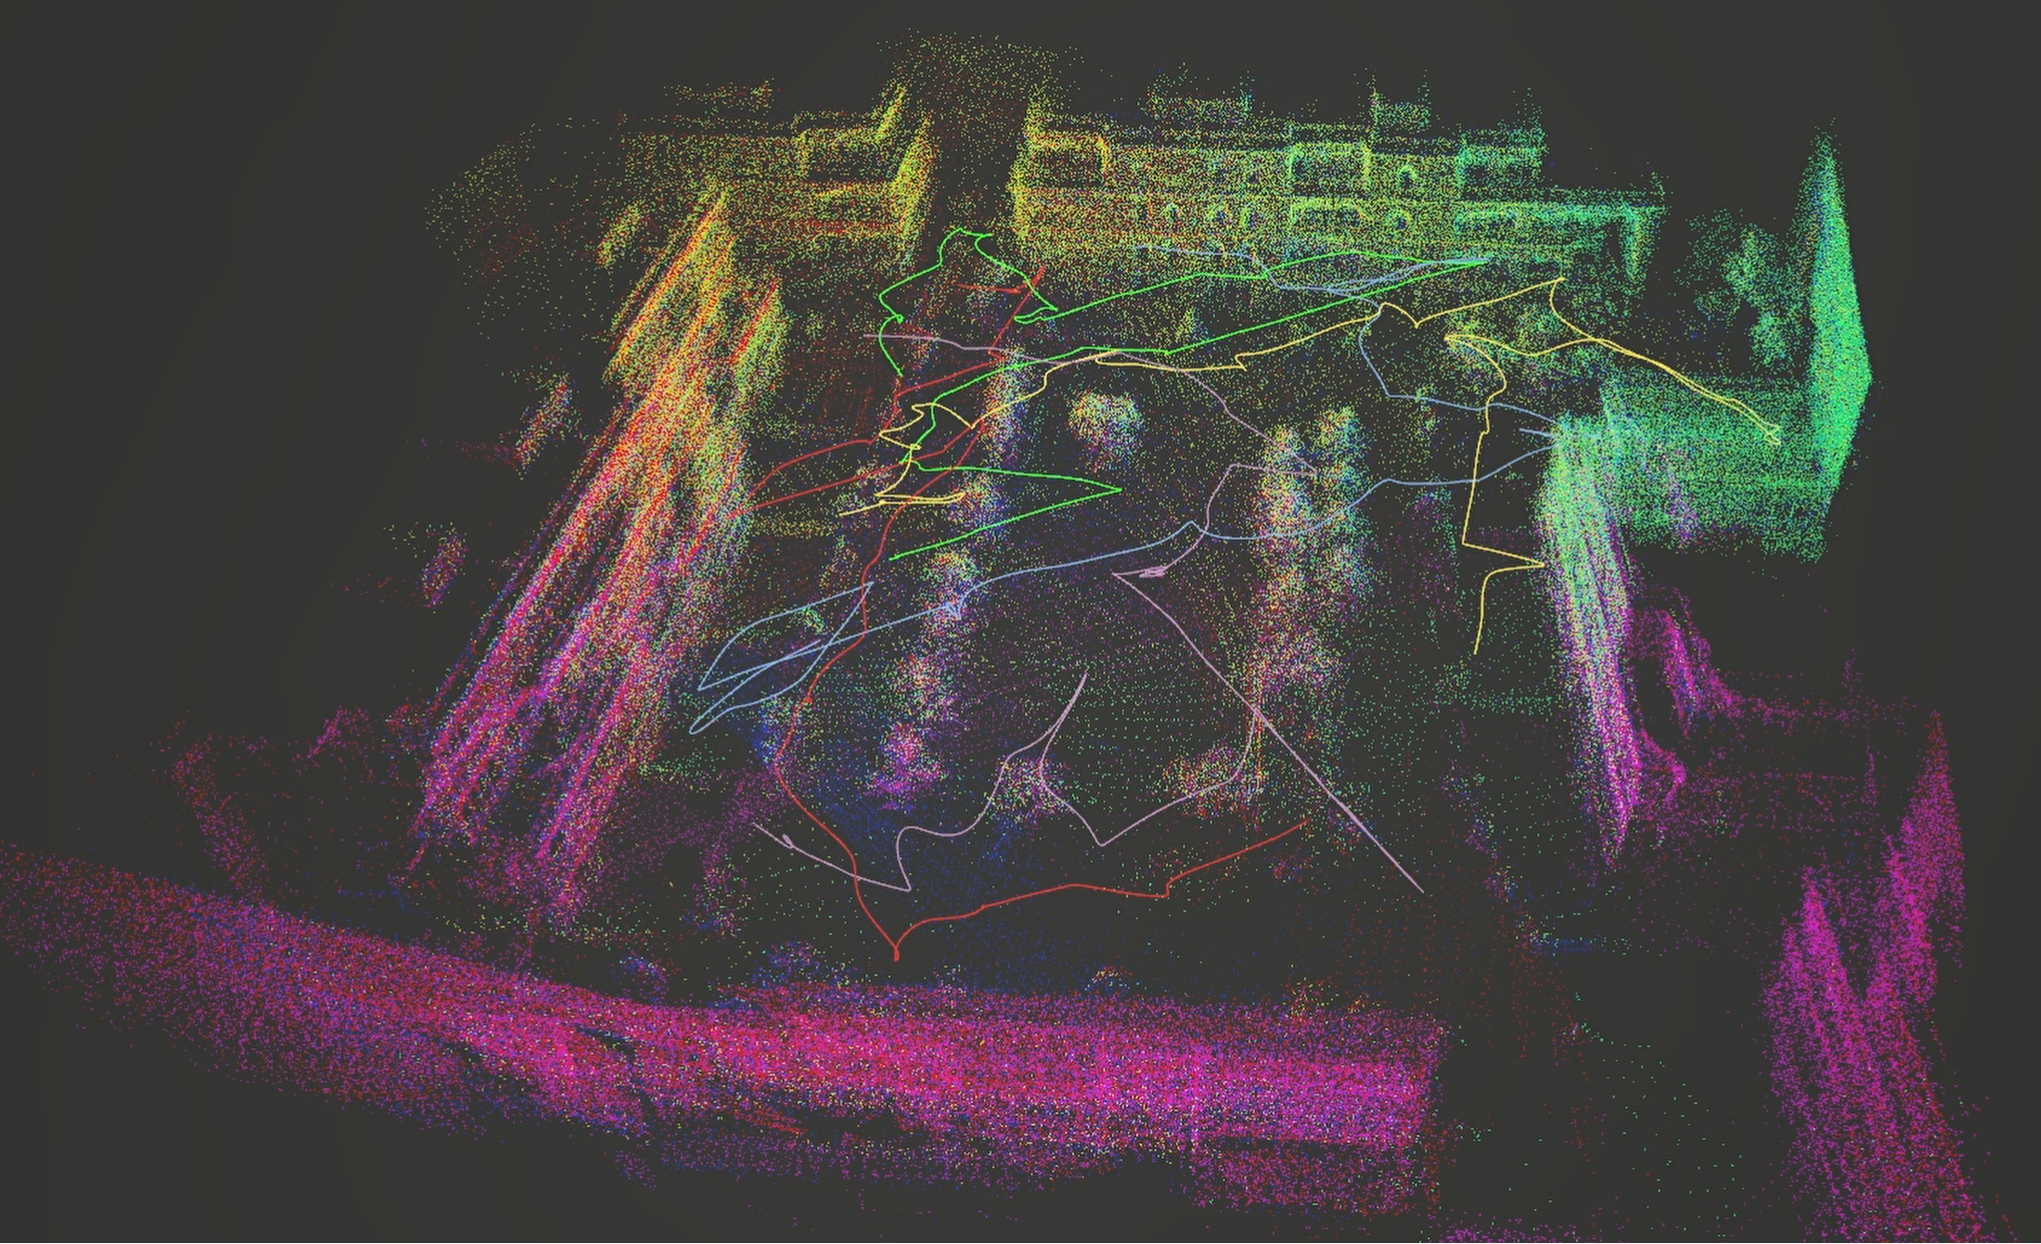
\includegraphics[width=0.32\columnwidth]{map_result_fame.png}}  
  \subfigure[]{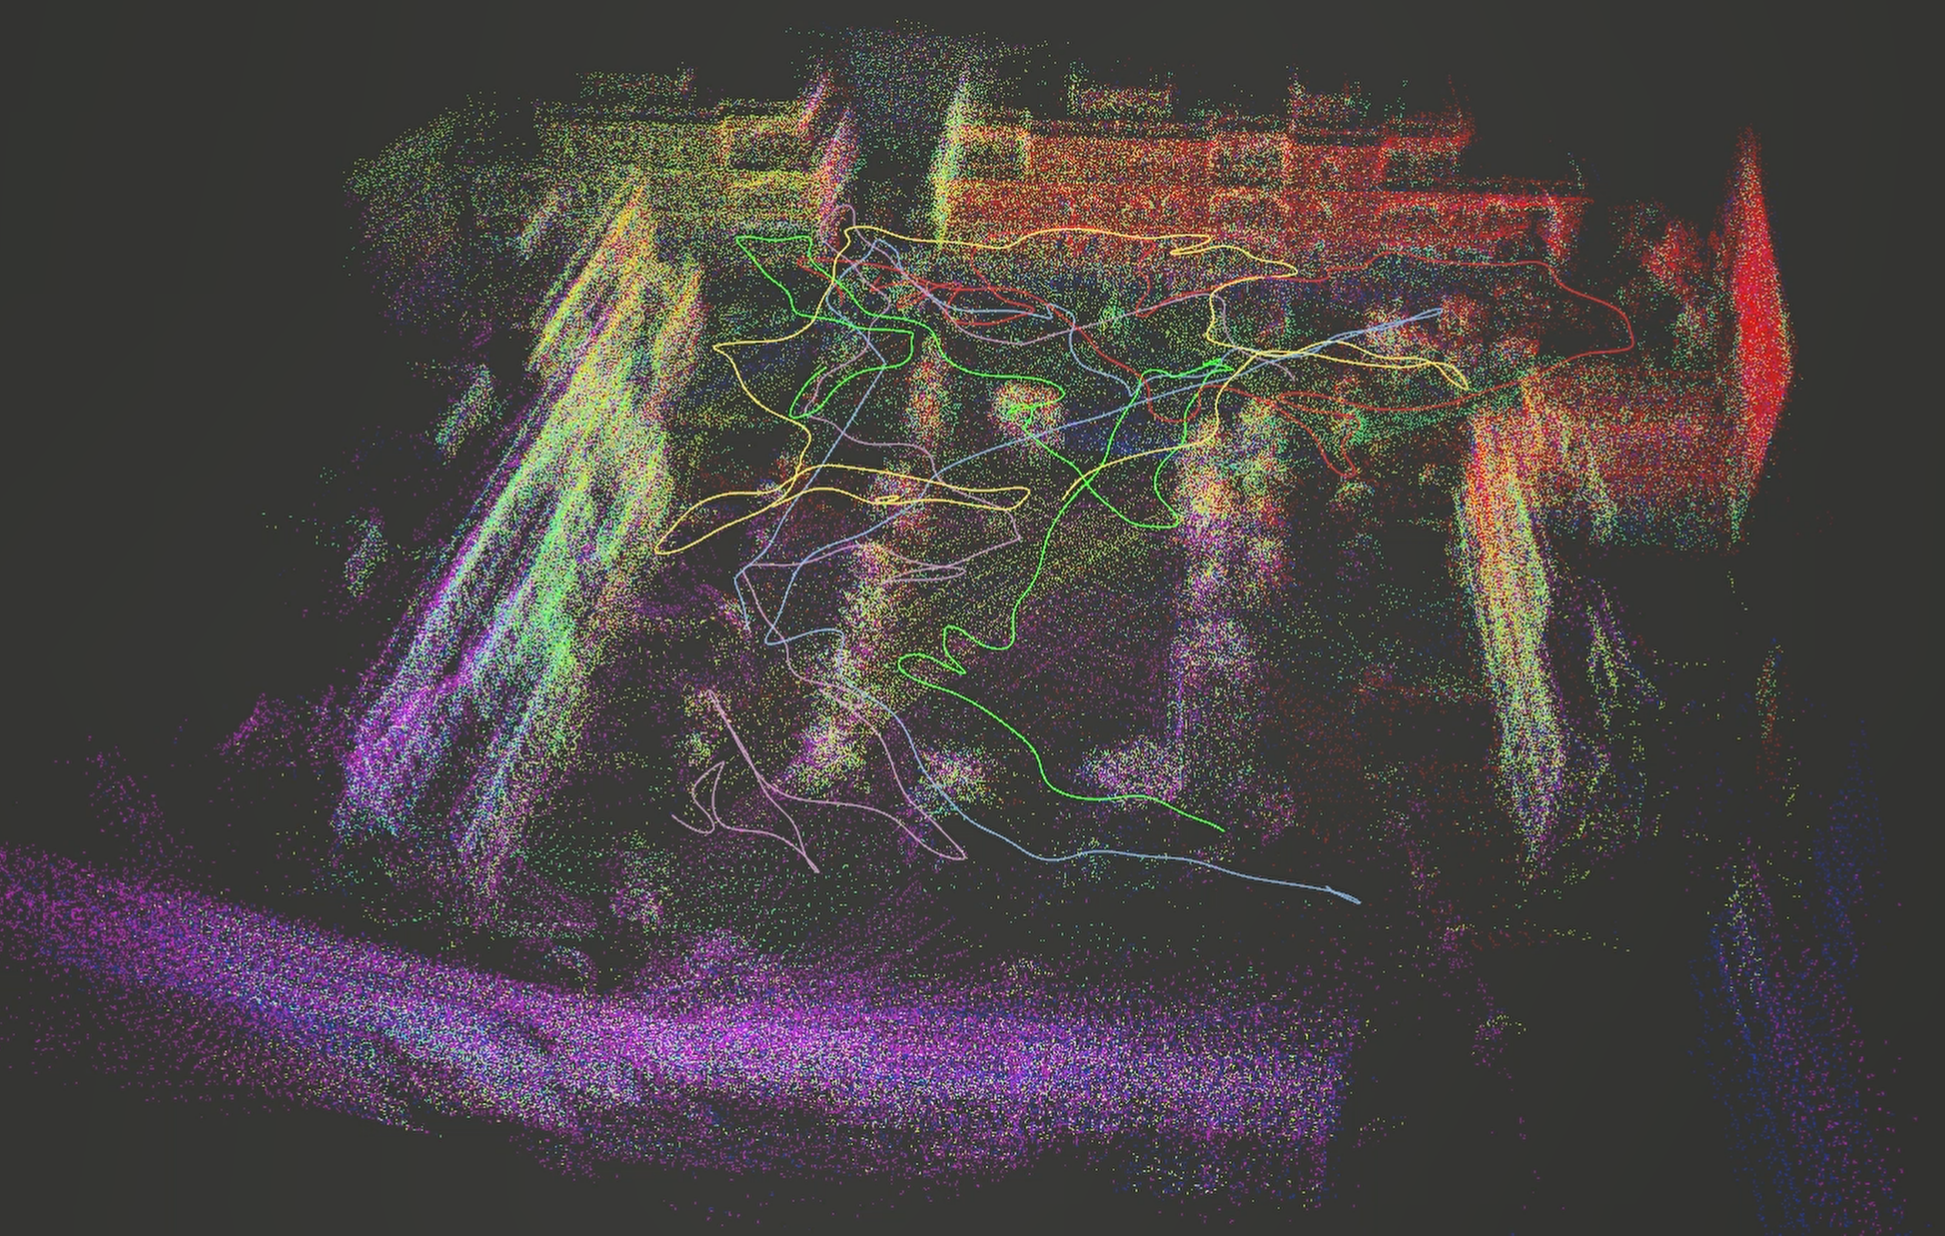
\includegraphics[width=0.32\columnwidth]{map_result_mapper.png}}  
  \caption{\label{fig_map_result} (a) The exploration result of RACER with 5 UAVs. (b) The exploration result of FAME with 5 UAVs. (c) The exploration result of MAPPER with 5 UAVs.}
  % \vspace{-0.6cm}
\end{figure}

To further evaluate the exploration efficiency and computational efficiency of the algorithms, we conducted extensive hardware-in-the-loop experiments in a real-world reconstruction scenario. Specifically, three algorithms were deployed on an RK3588S computing platform with 16GB of RAM, and all RK3588S platforms, along with the ground station, were connected to an AX6Pro router via wireless network. In the experiments, the number of drones was incrementally increased from 1 to 5, with each drone configuration being tested 5 times under the same conditions. We recorded the exploration time and the average computation time per exploration (which includes frontier clustering, viewpoint generation, task allocation, and trajectory planning), as shown in Figure 5. Additionally, Figure 6 presents the exploration results of the three algorithms in the real-world reconstruction scenario when 5 drones were used.
In Figure 5(a), it is clear that the proposed MAPPER algorithm required the least time to complete the exploration, finishing the task in just 88 seconds when 5 drones were used. The FAME algorithm, which overall performed second best, outperformed the RACER algorithm in all cases except when 5 drones were used. Observing Figure 5(b), the RACER algorithm had the lowest computational efficiency, while both MAPPER and FAME had comparable computational efficiency, significantly surpassing RACER. For the MAPPER algorithm, the increase in drone numbers did not have a significant impact on the computational time of the exploration planning. Regardless of the size of the drone fleet, MAPPER’s exploration planning computation time remained under 0.1 seconds, ensuring real-time feasibility for multi-drone systems.
Finally, as seen in Figure 6, all three algorithms successfully completed the exploration task in large-scale real-world reconstruction scenarios with 5 drones. In summary, the hardware-in-the-loop experiments further demonstrate the superior performance of the proposed MAPPER algorithm, laying a solid foundation for deploying this exploration algorithm in real-world applications.


\section{Conclusion}\label{sec:conclusion}
This paper presents an integrated task allocation and path planning method for multi-robot systems in cluttered environments. We introduce a novel path-planning approach called VES-Planner, which leverages a search based on the vertices of inflated obstacles to generate collision-free paths efficiently. Experimental results demonstrate that, on large-scale maps, VES-Planner achieves two orders of magnitude higher computational efficiency compared to current state-of-the-art path planners while producing collision-free paths with lengths close to optimal.
Building on the obstacle-avoidance paths generated by VES-Planner, we further address the detour cost during the robots' task execution. We propose a fast and accurate estimation method to approximate the robots' actual traveled distance, thereby enabling more efficient task allocation. Additionally, we improve the auction process in task allocation, reducing unnecessary repeated calculations and accelerating algorithm convergence without compromising solution quality. Finally, extensive simulation and real-world experiments validate the effectiveness and practicality of the proposed method.
In future work, we aim to address the dynamic collision problem among robots in cluttered environments while enhancing task allocation quality.

%		\section*{Acknowledgement}

\bibliography{ref}

\end{document}